\documentclass[11]{article}
\usepackage[utf8]{inputenc}

\title{Mémoire}
\author{bruno veraldi }
\date{June 2017}


\setlength{\headsep}{0.6in}

\usepackage[utf8]{inputenc}

\usepackage{color}
\usepackage[usenames,dvipsnames]{xcolor}

\usepackage{euscript}
\usepackage{amsmath}
\usepackage{amssymb}
\usepackage{amsfonts}
\usepackage{dsfont}
\usepackage{graphicx}
\usepackage{verbatim}
\usepackage[francais]{babel}
 \AddThinSpaceBeforeFootnotes 
\FrenchFootnotes 
\usepackage{epsfig}
\usepackage{thmbox}
\usepackage{graphicx}

\usepackage{amssymb}
\usepackage{caption}

\usepackage[final]{pdfpages}
\usepackage[export]{adjustbox}
\usepackage{afterpage}
\usepackage{emptypage}

\usepackage[toc,page]{appendix} 
\usepackage{a4wide}
\usepackage{csvsimple}
\newcommand{\R}{\mathbb{R}}
\newcommand{\Q}{\bf{Q}}
\usepackage{float,lscape}
\usepackage[nottoc]{tocbibind}

\usepackage[francais]{babel}
\usepackage[T1]{fontenc}
\usepackage{listings}
\usepackage{caption}
\usepackage{subcaption}

\usepackage[letterpaper, margin=1.5in]{geometry}






\usepackage{titlesec}

\setcounter{secnumdepth}{4}

\titleformat{\paragraph}
{\normalfont\normalsize\bfseries}{\theparagraph}{1em}{}
\titlespacing*{\paragraph}
{0pt}{3.25ex plus 1ex minus .2ex}{1.5ex plus .2ex}





\usepackage{fancyhdr}
\usepackage{lastpage}

\pagestyle{fancy}
\fancyhf{}
\fancyhead[LE,RO]{\leftmark}
\fancyfoot[LE,LO]{Bruno Veraldi \AuteurMemoire}
\fancyfoot[CE,CO]{Xamarin et l'écosystème Microsoft}
\fancyfoot[LE,RO]{Page \thepage/\pageref{LastPage}}


\renewcommand{\footrulewidth}{0.4pt} % Line at the footer visible

\newcommand{\HRule}{\rule{\linewidth}{0.5mm}}




\begin{document}
\begin{titlepage}
\begin{figure}[h]
    \begin{minipage}[c]{.16\linewidth}
        \centering
        
\includegraphics[width=4\textwidth]{logo-univ}
    \end{minipage}
    \hfill%
    \begin{minipage}[c]{.16\linewidth}
        \centering
        
\includegraphics{ufrSegmi}
    \end{minipage}
\end{figure}
\begin{center}

\noindent\rule{12cm}{0.4pt}
{ \huge \bfseries Mémoire   \\[0.4cm] }
\noindent\rule{12cm}{0.4pt}

\vspace{1cm}

\textsc{\Large \textbf{Master 2 :}  Méthodes Informatiques Appliquées à la Gestion des Entreprises }\\[0.5cm]
% Title

\vspace{0.5cm}

\textbf{\Large Xamarin et l'écosystème Microsoft est-il une solution pérenne
pour le développement d’applications mobiles cross-plateformes ?}\\[0.9cm]


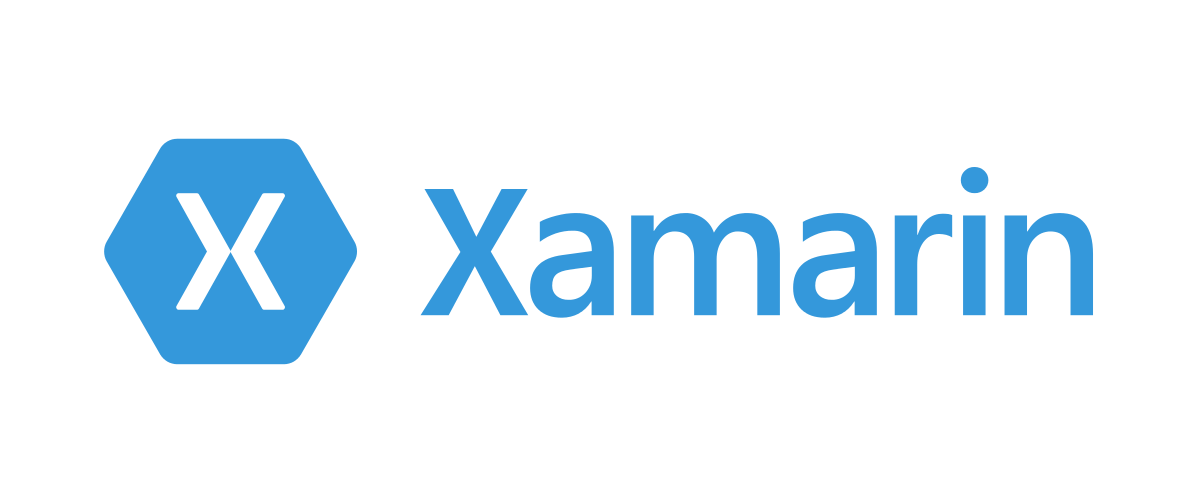
\includegraphics[width=0.6\textwidth]{xamarin-logo}~\\[1cm]


\Large {Tuteur : Souheib BAARIR}

\vspace{0.5cm}

\Large {Par : Bruno VERALDI} 

\Large {bruno.veraldi@gmail.com}

\vspace{0.5cm}

\Large {2017} 

\end{center}


\end{titlepage}
 
\newpage
\thispagestyle{empty}
\strut 

\newpage

\setcounter{page}{1}

\begin{center}
\textbf{\huge Remerciements}
\end{center}

\vspace{1.5cm}

\hspace{0.5cm} 

Durant mon master à l’université Paris Nanterre, j’ai eu l’opportunité de me découvrir un fort attrait pour la conception et la programmation d’application mobile. Celle-ci s'est établie par l’intermédiaire des cours dispensés ainsi que par le biais des projets réalisés au sein de la Junior entreprise de la formation. Grâce à cette expérience j’ai pu m’orienter vers le stage de mon choix en développement d’application mobile en Xamarin, ce qui me permet à l’heure actuelle d’acquérir de toutes nouvelles compétences sur cette technologie et son environnement bien distinct.

\vspace{0.5cm}

Pour cela je tiens à remercier : 

\vspace{0.5cm}

Monsieur Souheib BAARIR, tuteur de ce mémoire pour sa participation, son écoute ainsi que la liberté donnée dans le choix de mon sujet.

\vspace{0.5cm}

Monsieur Fabrice LEGOND-AUBRY pour les cours dispensés en Android.

\vspace{0.5cm}

Monsieur Nicolas MAYEUR, CEO de Mustanga pour m’avoir donné l’opportunité d’intégrer son entreprise ainsi que pour son écoute et pour les différentes tâches données me permettant d’avoir une meilleure vision de l’entreprise ainsi que de m’épanouir dans mon travail.

\vspace{0.5cm}

Monsieur Kevin JALAIS, consultant .NET / Xamarin pour sa disponibilité, son encadrement ainsi que la formation prodiguée tout au long de mon stage.

\newpage
\thispagestyle{empty}
\strut

\newpage
\setcounter{page}{2}
\tableofcontents

\thispagestyle{empty}

\newpage
\thispagestyle{empty}
\strut


\newpage
\thispagestyle{empty}
\begin{center}
\part{Introduction}
\setcounter{page}{5}
\noindent\rule{12cm}{0.4pt}
\end{center}

Le marché des applications mobiles sur smartphone est un monde en perpétuelle évolution et expansion. Cette expansion transparaît par la popularisation du smartphone ce qui a propulsé la vente de smartphones depuis 2009 jusqu’à atteindre une volumétrie de vente en million d’unités multiplié par 12,3 aujourd’hui; voir ci-dessous l’évolution du marché réalisé par l’international Data Corporation (IDC).


\begin{figure}[h]
    \centering
    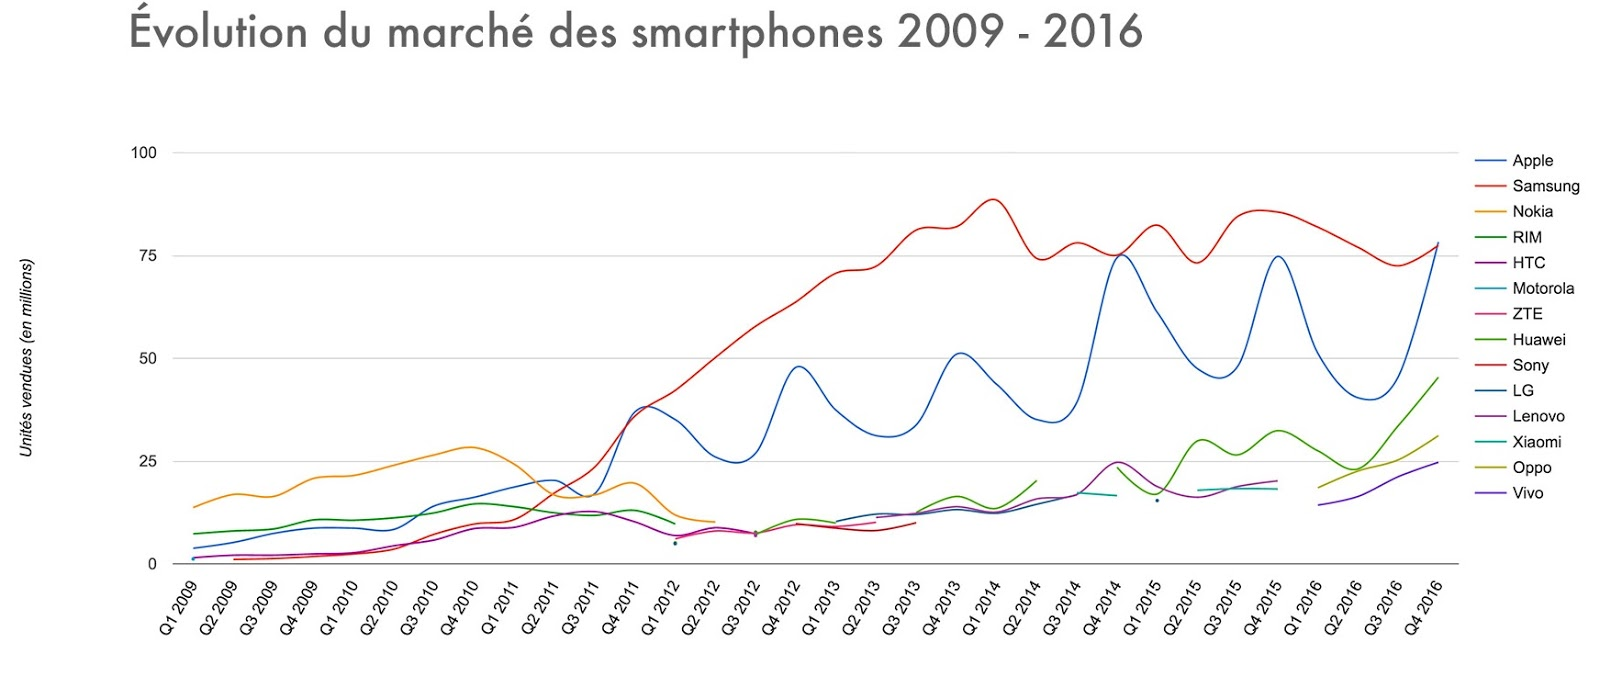
\includegraphics[width=1\textwidth]{evolution-market}
    \caption{Evolution du marché des smartphone 2009 - 2016}
    \label{bat}
\end{figure}

\vspace{0.5cm}

Par conséquent afin de cerner le marché des applications mobiles intéressons-nous à l’évolution du smartphone et ses dépendances en hardware, en technologies de téléphonies mobiles, en systèmes d’exploitation, en innovation ainsi que dans les solutions permettant leur développement.

 \vspace{0.5cm}
 
L’histoire du smartphone commence dès les années 90, avec la commercialisation en 1994 de l’IBM Simon, première ébauche du smartphone. Celui-ci bénéficiait d’un écran tactile ainsi que déjà de la majorité du socle applicatif de base que l’on retrouve de nos jours, tel que le service de messagerie, le carnet d’adresse, l’agenda avec gestion de rendez-vous, le traitement de texte pour les notes, l’horloge, la calculatrice et les jeux. Par la suite en 1997, Nokia mis sur le marché le 9000 Communicator, ajoutant aux fonctionnalités de base la précieuse navigation sur internet.

 \vspace{0.5cm}
 
En 2000, la 3G (troisième génération des normes de téléphonie) autorise les échanges de données et la voix sur le réseau ce qui permis aux différents constructeurs tels que Blackberry et Motorola avec son célèbre Razr V3 (2004) de démocratiser la navigation internet et l’accès aux contenus multimédia via téléphone. Quelques années plus tard en 2007, Nokia complète les éléments de base du smartphone avec son N95, bénéficiant d’un écran couleur, du Bluetooth, du WiFi, de la 3G et d’un appareil photo.

 \vspace{0.5cm}
 
La vraie révolution du smartphone et des applications mobiles est arrivée en 2008. Tout d’abord avec la date du 11 juin 2008 où Apple met en vente l’iPhone 3G qui devient rapidement le véritable smartphone de référence. De plus, un mois plus tard jour pour jour, Apple met à disposition une plateforme de téléchargement d’application en ligne, l’App Store; celle-ci va populariser la consommation d’application mobile et va par son intermédiaire permettre aux développeurs de proposer leurs propres applications.

 \vspace{0.5cm}
 
Après le succès mondial de l’iphone, les autres marques se sont tournées majoritairement vers l’OS Android, les autres plus tardivement vers Windows Phone. Le 22 octobre 2008 en même temps que l’ouverture de l’android Market le premier téléphone sous Android, le HTC Dream est commercialisé. A partir de cet instant les entreprises mettant sur le marché leurs smartphones sous l’OS Android et iOS pour Apple se vouent une concurrence féroce en mettant en avant tant bien le hardware et design du smartphone que la disponibilité d’applications mobiles dans leur store respectifs.
 
 
\newpage
\thispagestyle{empty}
\begin{center}
\part{Contexte et problématique}
\noindent\rule{12cm}{0.4pt}
\end{center}

A l’heure actuelle, nous constatons, grâce à l'Étude menée par l’entreprise Gartner ( voir figure 2 ) sur le taux d’utilisation et de la répartition du marché vis-à-vis des ventes mondiales de smartphone par système d’exploitation, que les 99,6\% du marché profite à Android et iOS. 

\vspace{0.5cm}


\begin{figure}[h]
    \centering
    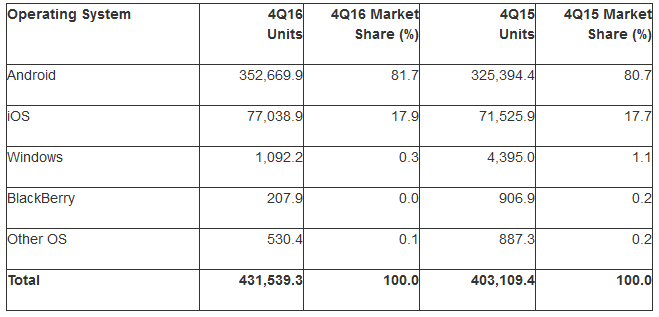
\includegraphics[width=1\textwidth]{gartner1}
    \caption{Ventes mondiales de smartphones par système d'exploitation (en milliers d'unités)}
    \label{bat2}
\end{figure}




Dès lors, dans ce contexte de domination totale du marché par ces OS, il devient nécessaire pour les entreprises de publier leurs applications sur les plateformes de téléchargement d’application en ligne de celles-ci, sous peine de se priver d’une importante part du marché. Par conséquent, l’une des problématiques courante du développement d’une application mobile est le déploiement de celle-ci sur au minimum les 2 plateformes qui sont l’App Store et le Play Store .

\vspace{0.5cm}

De plus, la conséquence directement lié à ce phénomène de domination, est la présence sur tout le globe d’utilisateurs de ces smartphones, d'où l’obligation pour les applications professionnelles d’être en capacité de fournir un service permettant une accessibilité rapide aux données tel que grâce à la géo-réplication des serveurs à travers le monde grâce au Cloud.

\vspace{0.5cm}

De surcroît, le processus de création d’une application mobile est souvent soumis à la contrainte de la stratégie d’un Time to market le plus réduit qui soit. Cette stratégie a pour objectif d’atteindre son marché le plus rapidement possible ainsi que de s’offrir un cadre d’amélioration continue par le jeu de l’agilité et des adaptations nécessaires afin de toujours mieux correspondre aux besoins des cibles, utilisateurs et clients.

\vspace{0.5cm}

Ainsi, les exigences du développement d’application mobile en terme de qualité sont devenues nombreuses et complexes car les applications doivent souvent :

\begin{itemize}
\item Etre développées dans des cycles courts
\item Exploiter au mieux les performances du matériel
\item Permettre une accessibilité mondialisée en temps réduit aux données externes
\item Bénéficier d’une bonne ergonomie et intuitivité
\item Etre design
\item Disposer d’une bonne maintenabilité
\item Avoir un excellent rapport qualité/prix
\end{itemize}

\vspace{0.5cm}

Afin de répondre à la problématique correspondant à ces exigences, des solutions technologiques ont émergé face au développement purement natif utilisant les langages de programmation Objective C ou Swift pour iOS, Java pour Android et C\# pour Microsoft. 
Ces solutions technologiques sont de deux types, nous avons d’un côté les frameworks HTML hybrides et de l’autre côté les frameworks natif cross-plateforme avec compilateur. Le principal avantage de ces solutions est leur volonté de fournir un outil permettant aux entreprises et développeurs de créer des applications mobiles tout en réduisant le temps de développement, le coût du projet et ce tout en bénéficiant d’une application de qualité.

\vspace{0.5cm}

Réalisant mon stage dans une entreprise spécialisée en développement d’application mobile en Xamarin j’ai souhaité développer la problématique suivante : 

\vspace{0.5cm}
 
 \begin{center}
\textbf{L’environnement Xamarin dans l'écosystème Microsoft 
est-il une solution pérenne pour le développement d’applications mobiles ?}
\end{center}

\vspace{0.5cm}



\newpage

\begin{center}
\part{Etat de l’art}
\noindent\rule{12cm}{0.4pt}
\end{center}

\setcounter{section}{0}

Aujourd’hui le marché du mobile est fragmenté en trois principales plateformes, Android, iOS, UWP. De part cette fragmentation si l’on souhaite développer une application native pour ces plateformes sans passer par une solution permettant le développement cross-plateforme il nous faut développer pour chaque Système d’exploitation avec son propre langage et technologies associés. Par conséquent il faut souvent associer une équipe par plateforme, assurer la gestion de celles-ci afin d’unifier le standard le l’application sur les différentes plateformes, assurer la maintenance sur chacune d’entre elles, et bien d’autres contraintes qui ne font qu’augmenter les coûts de l’application tout en ajoutant plus de complexité.

\vspace{0.5cm}

Afin de diminuer en complexité et permettre le développement rapide d’applications mobile à coûts faible ou modérés, des solutions technologiques ont émergés. Ces solutions, ce sont les frameworks et environnement de développement cross-plateformes.

\vspace{0.5cm}

Ainsi, nous allons dans ce chapitre mettre en lumière les différentes composantes liés aux solutions de développement d’application mobile cross-plateformes.


\section{Plateforme et systèmes d’exploitation mobiles}

Les systèmes d’exploitation ou Operating System (OS) sont un ensemble de programme fonctionnant conjointement dont le but est d’agir comme un intermédiaire, afin de permettre à un utilisateur d’interagir entre les logiciels et la machine.

\vspace{0.5cm}

Pour réaliser cela l’OS est principalement composé d’un noyau ou kernel permettant la gestion des composants du smartphone, la gestion des fichiers, la gestion de la mémoire allouée, les tâches et processus à opérer; d’un environnement d'exécution ou runtime pour l'exécution des programmes; et de bibliothèques logicielles utilisées par les programmes.

\vspace{0.5cm}

Xamarin permet le développement d’application sous 3 OS :

\begin{itemize}
\item Windows 10
\item Android
\item IOS
\end{itemize}

\subsection{Windows 10 et UWP}

Rendu disponible depuis le 29 juillet 2015, Windows 10 est un système d’exploitation très répandu puisque d’après la conférence de la Microsoft Build 2017 à Seattle il y aurait 500 millions d’appareil sous cet OS.
 
\vspace{0.5cm}

Toutefois Windows bénéficie d’une spécificité, par l’intermédiaire d’Universal Windows Platform (UWP) qui est la plateforme permettant de développer pour les appareils sous windows 10.
 
\vspace{0.5cm}

UWP n’est pas un système d’exploitation mais une plateforme d’application unifiée pour Windows 10. Cela signifie que l’on peut développer une application unique mais qui pourra être disponible sur tous les appareils bénéficiant de l’OS Windows 10 tel que les smartphones, tablettes, PC en fonction de la couche d’API utilisé. En effet, la limite lié à la disponibilité de l’application sur les différentes plateformes windows est liée aux API ciblés, par exemple si on cible les API spécifiques à HoloLens, l’application ne sera disponible que sur ce matériel.
 
\vspace{0.5cm}

UWP s’appuie tout d’abord sur une famille universelle d’appareil tel que les PC, les téléphones (voir figure 3).

\vspace{0.5cm}

\begin{figure}[h]
    \centering
    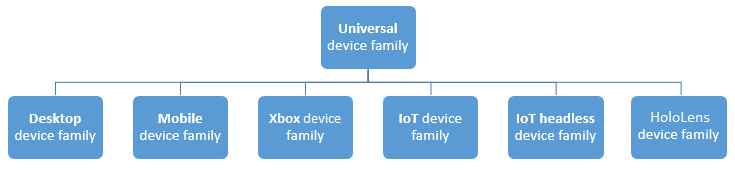
\includegraphics[width=1\textwidth]{uwp}
    \caption{La famille universelle d'UWP}
    \label{bat}
\end{figure}


L’avantage de cette famille d’appareils universels est de pouvoir déployer une application qui fonctionnera avec certitude avec les API dans la catégorie d’appareil ciblée car chaque famille bénéficie de ses propres APIs exceptée la famille universelle qui est générique. Ainsi chaque famille bénéficie d’APIs distinctes et d’APIs qui héritent de la famille universelle fonctionnant sur tous les appareils Windows.
 
 \vspace{0.5cm}
 
De plus UWP utilise un Windows Core commun permettant de bénéficier d’une source commune tel que le noyau windows. Par ailleurs, l’interface utilisateur a aussi été unifiée avec un framework XAML et un framework HTML.


\subsection{Android}

Android est un OS open source actuellement développé par Google dont la première version commerciale stable 1.0 a été officiellement mis à disposition le 23 septembre 2008. Un mois plus tard est commercialisé l’HTC Dream, le premier smartphone android. Depuis, il c’est succédé pas moins de 10 versions différentes d’Android portant un nom de sucrerie différent à chaque version, la dernière en date est celle du 10 mars 2016, la version “Nougat”. Grâce à son évolution Android est devenu de nos jours l’OS mobile le plus utilisé au monde.

\vspace{0.5cm}

Android est un OS bénéficiant d’une architecture contenant de nombreux composants, nous allons étudier ci-après les principaux composants de celui-ci.

\begin{figure}[h]
    \centering
    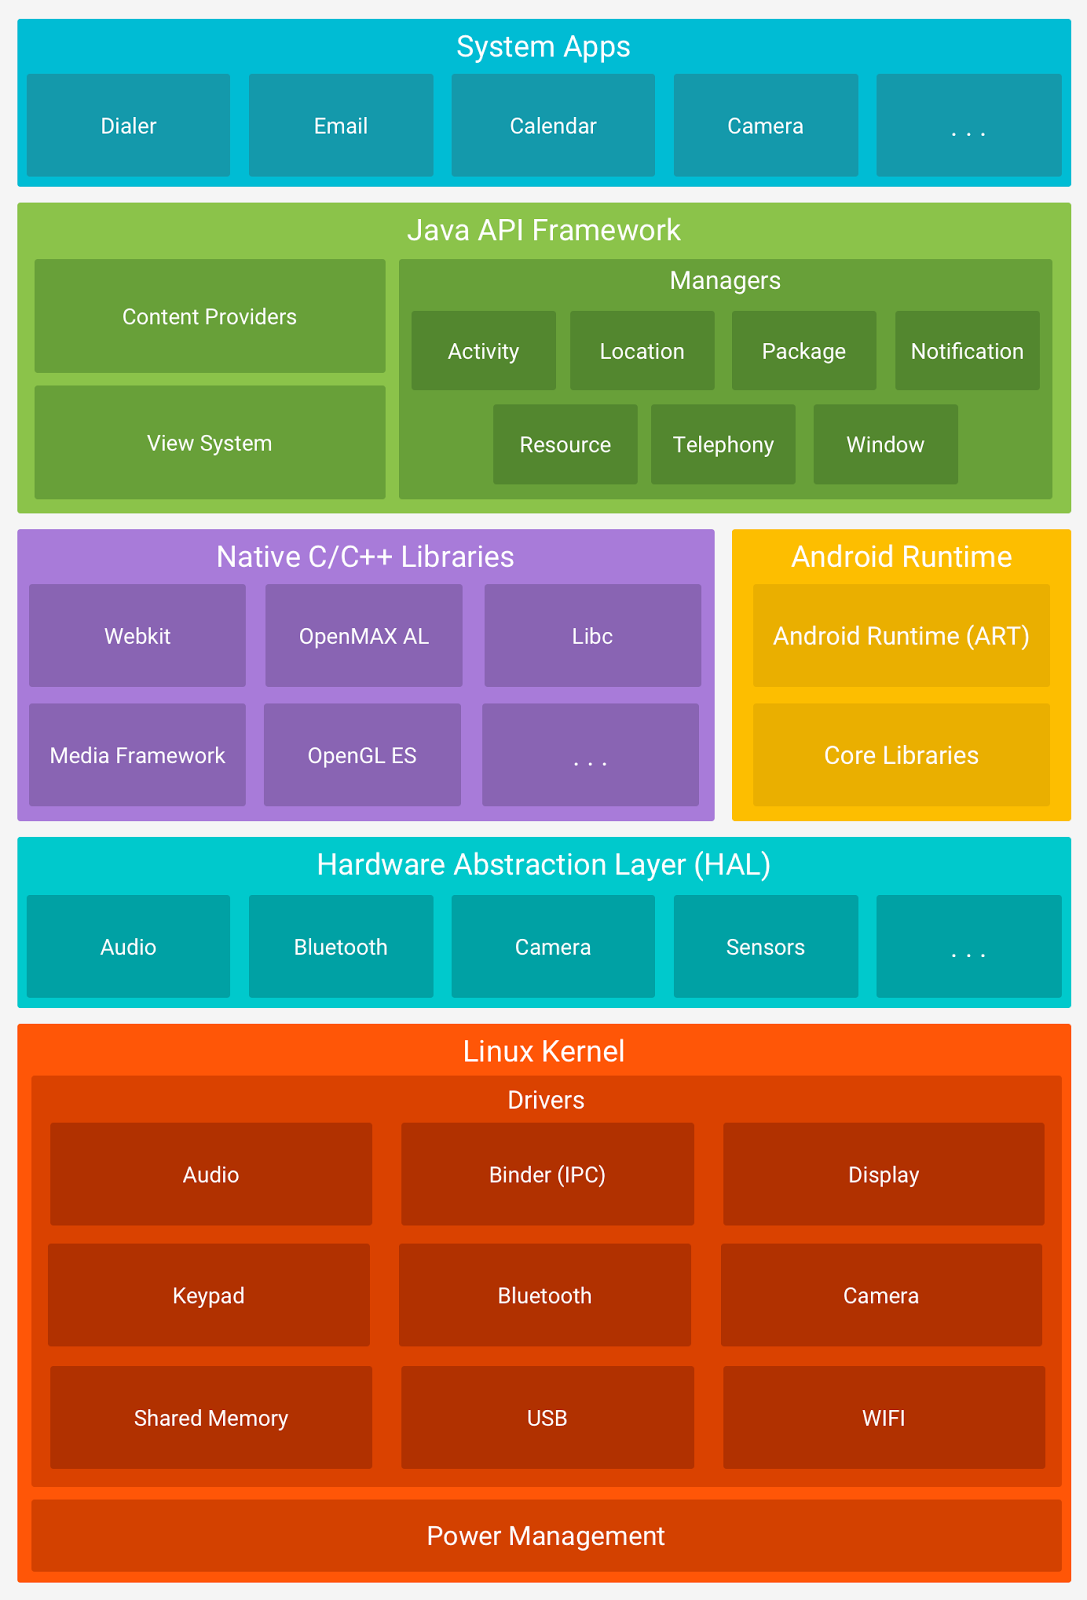
\includegraphics[width=0.6\textwidth]{androidos}
    \caption{Android OS architecture}
    \label{bat}
\end{figure}


\subsubsection{Un coeur Linux}

Le coeur linux est la fondation de la plateforme Android, elle comprend l’Android Runtime (ART) pour les fonctionnalités telles que le threading et la gestion de la mémoire.
Le choix d’un noyau Linux n’est pas anodin car celui-ci est bien connu des constructeurs, par conséquent ceux-ci peuvent facilement créer leur smartphone tout en développant leurs pilotes matériels correspondant. Par ailleurs, le coeur linux est éprouvé et comprends de base d’importantes fonctionnalités tel que celles de sécurité.


\subsubsection{La couche d’abstraction matérielle}

La couche d'abstraction matérielle (HAL)  a pour objectif de fournir les interfaces standardisées afin d’exposer les fonctionnalités matérielles propres à chaque smartphone Android au framework d’API Java.
Cette couche est composée de modules de bibliothèques propres au composant matériel tel que le Bluetooth, ainsi chaque composant implique une interface standardisée.
 
 \vspace{0.5cm}
 
Cette couche fonctionne conjointement avec le framework d’API Java, c’est à dire qu'à chaque appel à un composant matériel via l’API, l’OS Android charge le module de la bibliothèque correspondante.


\subsubsection{L’Android Runtime}

Depuis la version 5.0 d’Android (API 21, “Lollipop”) chaque application bénéficie maintenant de son propre processus et instance dans l’Android Runtime (ART), celui-ci remplace l’ancien Dalvik.
 
L’Android Runtime comprend donc l’Android Runtime (ART) qui contient :

\begin{itemize}
\item Un compilateur Ahead Of-Time (AOT) et Just-In-Time (JIT) pour une exécution plus performante car le code est précompilé
\item Un garbage collector optimisé
\item Un support de débogage pour les exceptions, les rapports de crash
\end{itemize}

 \vspace{0.5cm}
 
De plus Android inclut un ensemble de bibliothèques pour l'exécution ce qui fournit la plupart des fonctionnalités utilisés par le framework d’API Java.

\subsubsection{Les bibliothèques C/C++ Native}
Les bibliothèques C/C++ native sont utilisées par les principaux composants du système tel que ART et HAL. Ces bibliothèques sont aussi accessibles via le framework d’API Java qui expose aux applications un certain nombre des fonctionnalités de ces bibliothèques natives, c’est entre autre le cas d’OpenGL.

\subsubsection{Le framework d’API Java}
Les APIs exposé par le framework d’android a pour objectif de rendre disponible les fonctionnalités du système d’exploitation d’Android.
Les APIs de ce framework forment des blocs de construction réutilisables permettant la création d'application mobiles.

 \vspace{0.5cm}
 
Le framework d’API Java contient :
\begin{itemize}
\item Un système de vue permettant la création d’interface utilisateur tel que les ListView, les zones de texte, les grilles ou encore les boutons.
\item Un gestionnaire de ressources permettant l’accessibilité aux ressources autres que celles du code.
\item Un système de gestion de notification afin d’afficher les alertes liées aux applications.
\item Un gestionnaire d’activité pour la gestion du cycle de vie des applications
\item Un fournisseur de contenu permettant aux applications d’accéder aux données des autres applications tel que par exemple l’accès aux contacts et leurs données.
\end{itemize}

\subsubsection{Les applications système}
Les applications systèmes proposées par l’OS Android sont nombreuses, elles contiennent entre autres la navigation internet, l’email, la messagerie SMS, le calendrier, les contacts.
Les applications systèmes utilisent les mêmes fonctionnalités exposées par le framework d’API Java que celle d’une application non système.
L'objectif des applications système mis à part la fourniture d’un jeu d’application de base à l’utilisateur final, est de permettre aux développeurs la réutilisation des fonctionnalités de base de ces applications tel que par exemple l’envois de SMS.

\subsection{iOS}
iOS est un OS mobile développé par Apple à destination des appareils iPhone, iPad et iPod Touch.
Sa première version iOS 1 est apparue le 29 Juin 2007 avec la sortie de l’iPhone 2G. Depuis de nombreuses autres versions sont sorties jusqu’à actuellement la version 10.3.2.
 
 \vspace{0.5cm}
 
iOS bénéficie d’une architecture comportant quatre couches que nous allons détailler ci-après.

\begin{figure}[h]
    \centering
    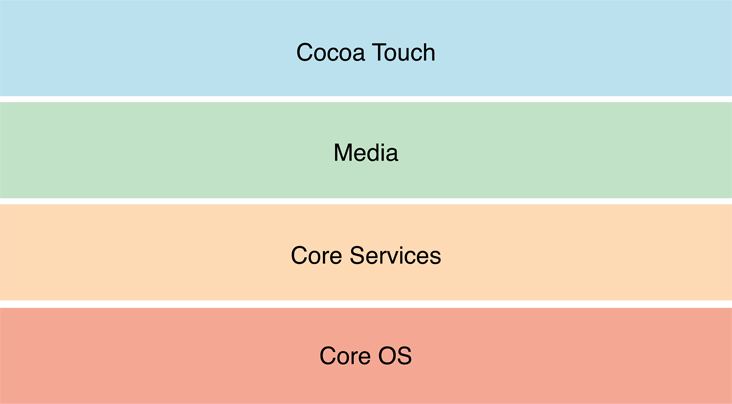
\includegraphics[width=0.7\textwidth]{ios-arch}
    \caption{Architecture iOS}
    \label{bat}
\end{figure}


\subsubsection{La couche Core OS}
La couche Core OS est la couche la plus profonde de iOS, elle contient le socle de base de celui-ci. Ce socle se décompose en plusieurs composants tels que le noyau d’OS X, le gestionnaire du processeur en fonction de sa charge et de la batterie, le système de bibliothèques.
  
 \vspace{0.5cm}
 
Ainsi le rôle de la couche Core OS est de gérer et fournir une variété de services, tel que le réseau ainsi que les fondamentaux des systèmes d’exploitation tels que la gestion de la mémoire.

\subsubsection{La couche Core Services}
La couche Core Services a comme objectif de mettre à disposition des API permettant une gestion du système plus poussée. On y retrouve entre autre la gestion des collections, la géolocalisation, les accès fichiers.

\subsubsection{La couche Média}
La couche Média a pour objectif la gestion des données multimédias, elle est composée de nombreux composant tels que le Core Audio, la gestion des formats d’image, un moteur graphique.

\subsubsection{La couche Cocoa Touch}
Cette couche est adaptée à l’interface Multi-touch d’iOS et contient les fonctionnalités en terme de gestion des événements tel que le Multi-touch, l’accéléromètre ou encore de l’utilisation de l’appareil photo.


\section{Les plateformes de téléchargement d’applications}
Pour chaque application mobile développée celle-ci ne pourra être rendue disponible que via la plateforme de téléchargement d’application en ligne de l’OS concerné, soit :

\begin{itemize}
\item Windows Store pour Windows 10
\item Google Play pour Android
\item l’App Store pour IOS 
\end{itemize}
  
 \vspace{0.5cm}
 
Par conséquent il est important de prendre en considération le facteur des stores dans le développement des applications mobiles tant ceux-ci peuvent imposer de nombreuses contrainte tant à l’acceptation des applications sur leurs stores.


\subsection{Windows Store}
Windows Store existe depuis le 11 juillet 2011, il avait à l’origine pour objectif de proposer des applications à destination des PCs uniquement, puis en 2015 il a fusionné avec Windows Phone Store afin de réunir les applications tablettes, smartphones, PC et console, car grâce à UWP les applications développées peuvent maintenant être compatible indifféremment avec toutes les plateformes.
   
 \vspace{0.5cm}
 
La publication d’applications via Windows Store s’effectue via un compte développeur Microsoft personnel facturé 99\$ non renouvelable, valide à vie.

\subsection{Google Play}
Google Play est la boutique d’Android, elle est née le 6 mars 2012 de la fusion de android Market, Google Movies, Google Music et Google ebookstore. La volontée de google est de centraliser et rendre facilement disponible les différents produits par l’intermédiaire d’un unique service. Google Play est la plus grosse boutique d’application du monde avec ses 2,8 millions d’applications disponibles en mars 2017 (voir figure ci-dessous).

\begin{figure}[h]
    \centering
    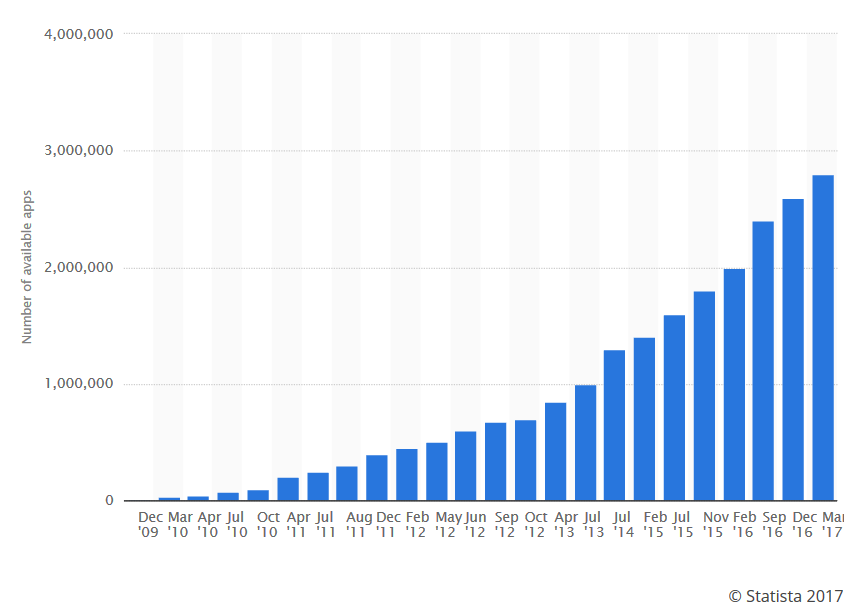
\includegraphics[width=0.9\textwidth]{histo-google}
    \caption{Histogramme Google Play}
    \label{bat}
\end{figure}
   
 \vspace{0.5cm}
 
La publication d’application via Google Play s’effectue via le compte personnel de la Google Play Console facturé 25\$ non renouvelable, valide à vie.

\subsection{App Store}
L’App Store, lancée par Apple depuis le 11 juillet 2008 est la boutique à destination des mobiles sous iOS.
    
 \vspace{0.5cm}
 
La publication d’une application sur l’App Store est une procédure plus complexe que les autres plateformes puisque Apple utilise une logique différente, elle ne s’adresse pas aux développeurs, mais aux entreprises. Par conséquent, pour publier une application il faut bénéficier d’un compte disponible uniquement pour l’entreprise, ce compte est facturé 99\$ par an. L’avantage de ce système est que l’on peut attacher autant de développeurs, testeurs que l’on souhaite via leur interface de gestion d’application Itunes connect.


\section{Les frameworks et environnements de développement cross-plateformes}
Pour développer une application mobile, il existe principalement 2 types de solutions que nous allons définir ci-après, tout d’abord nous avons le développement pur natif puis nous avons le développement cross-plateforme comprenant le développement hybride et le développement cross-plateforme natif.

\subsection{Le développement cross-plateforme}
Le développement cross-plateforme répond à la problématique du développement d’une même application à destination de périphériques différents tels que les smartphones et tablettes et de plateformes distinctes tel que Windows 10, Android ou iOS. La stratégie du développement cross-plateforme est de réduire les technologies langages employés, mutualiser et rendre le code réutilisable quel que soit la plateforme et ce afin de diminuer la charge de travail, le temps de réalisation, la complexité et par conséquent les coût de la création d’une application. 

\subsection{Les plateformes de développement d’application mobile}
Grâce au fort potentiel du développement cross-plateforme de nombreuses solutions ont émergés face au développement purement natif. Plusieurs types de développement existe, nous allons ici expliciter ces différents types.

\subsubsection{Le développement Natif}
Le développement d’application mobile en natif permet d’être au plus près des capacités du mobile et de son OS. Par conséquent les performances en natif avec un code optimisé seront optimales car on bénéficie d’un accès direct aux fonctions spécifiques et APIs des plateformes.
Néanmoins, cette solution est coûteuse car elle nécessite pour chaque plateforme l’utilisation de langages et d’environnements spécifiques aux plateformes, soit :
\begin{itemize}
\item Pour WPF (Windows 10) : l’environnement Visual Studio et le langage C\#.
\item Pour Android : l’environnement Android Studio et le langage Java.
\item Pour iOS : l’environnement Xcode et le langage Objective C ou Swift , avec de surcroît l’obligation de développer sur du matériel Apple.
\end{itemize}

\subsubsection{Le développement Hybride}
les applications dites hybrides s’appuient sur des frameworks tel que Ionic et PhoneGap basé sur Apache Cordova et emploient les langages Javascript, HTML5, CSS3. 
     
 \vspace{0.5cm}
 
Le principe de fonctionnement du développement d'application mobile hybride est de créer une application mobile native contenant une WebView.
     
 \vspace{0.5cm}
 
La WebView est une fenêtre du navigateur web contenue dans l'application, c'est elle qui va permettre le traitement du code et leur affichage.
     
 \vspace{0.5cm}
 
Les navigateurs utilisés changent en fonction de l'OS du smartphone, cela sera Chromium pour Android, Safari pour iOS et Edge pour Windows 10.
     
 \vspace{0.5cm}
 
Par ailleurs, Apache Cordova étends les possibilités d'interaction avec le mobile en permettant l'accès à un certain nombre de fonctionnalités natives tel que par le biais des plugins.
     
 \vspace{0.5cm}
 
Les principaux avantages de cette solution est le temps de développement court et donc les faibles coûts en développement ainsi que sa maturité, par conséquent c’est la solution parfaite pour l’établissement d’un produit minimum viable (MVP). 
Toutefois son inconvénient est liée à sa dépendance au navigateur tel que l’absence d’accessibilité à l’application en étant hors ligne, les différents comportements en fonction des smartphones, les performances, l’interface utilisateur ainsi que la lente adoption des nouvelles versions des différentes plateformes.


\subsubsection{Le développement Cross-plateforme natif}
les applications cross-plateforme compilés en natif ont pour volonté de proposer une expérience se rapprochant au plus près des performances natives du mobile. Celles-ci s'appuient sur des frameworks/compilateur tel que Titanium, React Native employant le langage Javascript ou encore Xamarin employant le langage C\# que nous allons étudier ci-après.


\section{L'environnement de développement Xamarin}
Xamarin est une technologie qui a pour objectif de produire des applications mobiles natives tout en permettant l'écriture d’un code partagé/unique fonctionnant sur les plateformes mobiles iOS, Android et Windows. C’est ainsi que Xamarin propose d’utiliser un même langage, les mêmes APIs  et structures de données.
     
 \vspace{0.5cm}
 
De plus selon Xamarin la moyenne de partage du code des applications sur les différentes plateformes de développement mobile est établie à 75\%.
     
 \vspace{0.5cm}
 
Voyons ci-après le fonctionnement de cette technologie ainsi que sa composition.

\subsection{Le code C\#}
Le langage utilisé en Xamarin est le C\#, c’est un langage de programmation orienté objet commercialisé par Microsoft depuis 2002. Le C\# est un langage mature profitant d’une constante évolution. Actuellement à la version 6.0, le C\# est utilisé avec le framework .NET ce qui lui permet de proposer comparés à ses concurrents des fonctionnalités sophistiquées tel que par exemple la généricité et les types dynamiques.
 
\subsection{Le XAML et le code behind pour les interfaces}
Le XAML ou eXtensible Application Markup Language est un langage basé sur le XML (Extensible Markup Language) qui a pour objectif de fournir aux développeurs un langage facilement éditable et réutilisable pour la création d’Interfaces Utilisateurs (UI).
      
 \vspace{0.5cm}
 
Une fois les UI crée en XAML le fonctionnement est le suivant. Lors de la compilation Un parser vient lire les fichiers XAML afin d’instancier les objets correspondants. Cela va générer automatiquement les classes et les enregistrer dans un projet xamarin dans le dossier “obj/debug”, ces classes issues de la génération bénéficient de l’extension tel par exemple : obj/debug/maPage.xaml.g.cs.
      
 \vspace{0.5cm}
 
L’intérêt du XAML est que ces classes générées sont définies en partial ce qui signifie qu’une partie du code se situe dans cette classe, et que l’autre partie partie se situe ailleurs, en l'occurrence dans le code-behind. Le Code-behind quand à lui permet d’implémenter le comportement des différents éléments de la page tel que les boutons ou encore les événements.


\subsection{Le framework .Net Mono}
Xamarin s’appuie sur la plateforme Mono qui est l’implémentation cross-plateforme des fonctionnalités du framework de Microsoft .NET basé sur le Common Language Runtime (CLR). 
Ainsi le framework Mono porte le CLR avec un compilateur sur les plateformes Android et iOS permettant aux applications d’être compilés sur ces environnements.

\subsection{La couverture des APIs d’iOS et Android}
Afin de bénéficier des performances natives d’Android et iOS, Xamarin expose les APIs natives au C\# par l’intermédiaire des librairies Xamarin.Android et Xamarin.iOS.
Cela a été rendu possible grâce aux liaisons 1 à 1 ou one-to-one bindings, ainsi grâce à ces liaisons 100\% des API d’iOS et Android ont étés couvertes donnant accès à toutes les fonctionnalités de ces OS pour le développement.

\subsection{Le partage de code}
La force de xamarin est son système de partage de code afin de bénéficier un large socle commun aux diverses plateformes. Ce socle est subdivisé en 3 couches (voir figure 7), une couche comprenant le code comportant la logique de l’application, une couche comprenant le code de l’UI et une couche comprenant le code des implémentations spécifiques aux plateformes.   

\begin{figure}[h]
    \centering
    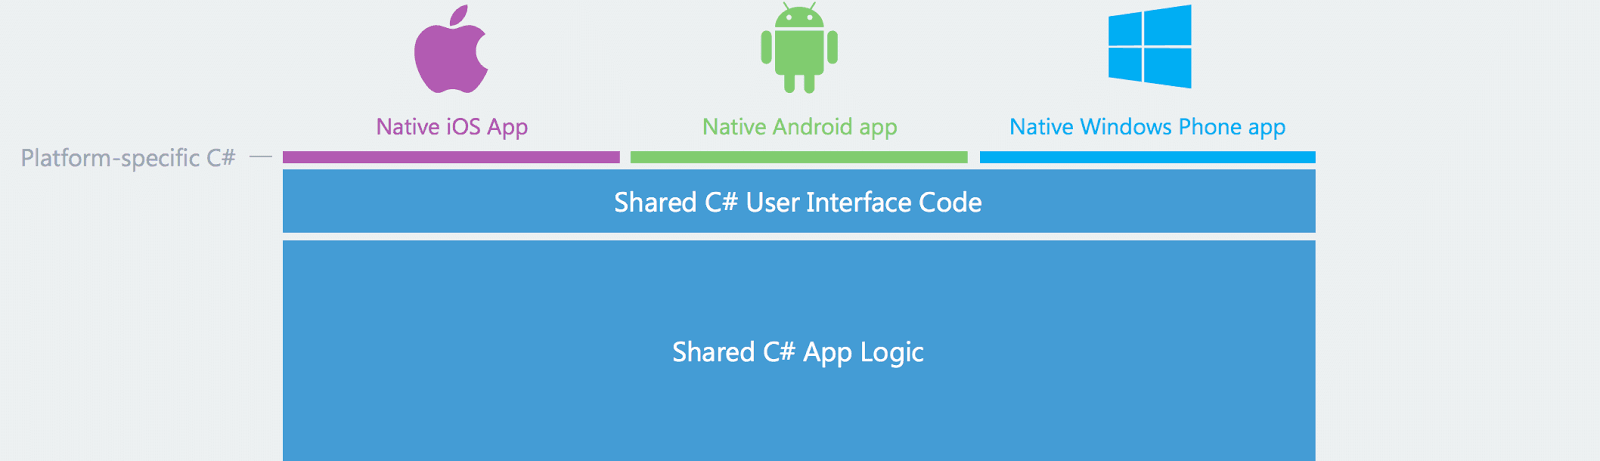
\includegraphics[width=0.9\textwidth]{code-share}
    \caption{Plateforme Xamarin}
    \label{bat}
\end{figure}

 \vspace{0.5cm}
 
 Pour réaliser cela il existe trois différentes stratégies pour partager le code entre les applications cross-plateformes vis-à-vis du code comportant la logique de l’application.

 \vspace{0.5cm}
 
 Puis, nous avons deux approches de développement en Xamarin permettant ou non de partager le code relatif aux interfaces des applications.

\subsubsection{Les stratégies de partage de code entre les plateformes}
L'objectif de la stratégie de partage de code est de soutenir l'architecture (voir figure 8 ci-dessous), où une base de code unique peut être utilisée par plusieurs plates-formes.

\begin{figure}[h]
    \centering
    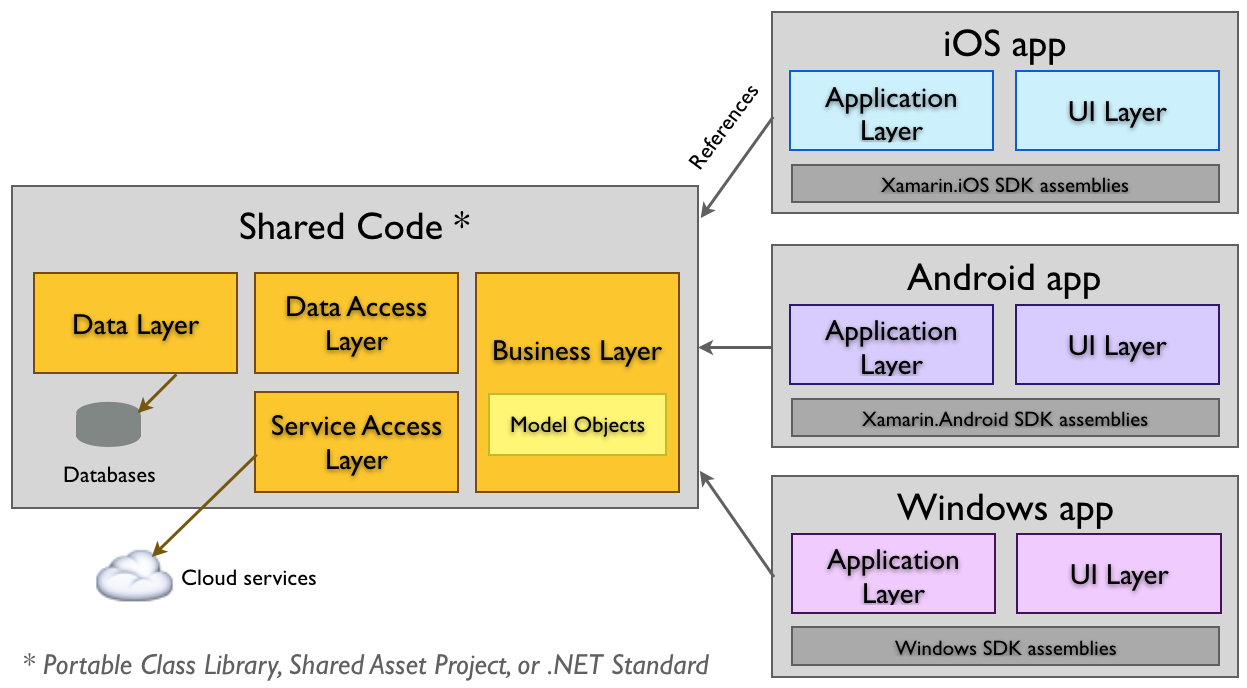
\includegraphics[width=1\textwidth]{arch-share}
    \caption{Stratégie de partage de code}
    \label{bat}
\end{figure}


\subsubsection{Le partage avec Shared Projects}
L'approche la plus simple pour partager le code consiste à utiliser un Shared Projects.
 
 \vspace{0.5cm}
 
L’idée de l'architecture d’un Shared Project est que chaque projet inclut tous les fichiers sources partagés du Shared Code tel que le Data Layer, le Data Access Layer, le Service Access Layer et le Business Layer.
 
 \vspace{0.5cm}
 
L’avantage de cette solution est qu’elle permet de partager du code sur plusieurs projets et que ce code peut être ciblé sur un plateforme spécifique en utilisant les directive du compilateur par exemple avec "\#if \_\_ANDROID\_\_" ou encore "\#if \_\_IOS\_\_". Par ailleurs les projets peuvent inclure des références spécifiques à la plateforme concernée. Toutefois la complexité d’un Shared Projects augmente car le code spécifique écrit pour toutes les plateformes est fondu dans les mêmes fichiers ce qui rend le code moins maintenable.
 
 \vspace{0.5cm}
 
Cette solution est destinée uniquement au partage de code dans les applications mobiles et non à la distribution à d'autres développeurs.


\subsubsection{Le partage avec Protable Class Libraries}
Utiliser un projet en Portable Class Libraries ou PCL va permettre au développeur d’écrire tout le code une seule fois dans une bibliothèque de classes portable qui sera partagé entre les plateformes. L’avantage est que cette bibliothèque PCL sera compatible avec toutes les plateformes et qu’elle ne nécessite aucune directive au compilateur.
  
 \vspace{0.5cm}
 
Ici il existe une subtilité d'accessibilité avec le code spécifique d’une plateforme. Celle-ci réside dans la définition d’une interface dont dépendent les projets des plateformes natives, puis d’utiliser l’injection de dépendances pour injecter la classe. Grâce à cette solution nous avons accès au code spécifique de la plateforme désirée à partir de n’importe quel PCL référencée par deux projets. 


\subsubsection{Le partage avec .NET Standard Libraries}
Les projets .NET Standard fonctionnent de manière similaire aux PCL, nécessitant l'utilisation d'Interfaces pour injecter des fonctionnalités spécifiques à la plate-forme.
   
 \vspace{0.5cm}
 
La .NET Standard Librairies est très similaire à PCL, mais bénéficie d’un plus grand nombre de classes de la Base Class Libraries ainsi qu’un modèle plus simple pour le support de plate-forme.


\subsubsection{Les approches de développement en Xamarin}
En Xamarin nous avons la possibilité de développer le code de deux manières en fonction de nos objectifs. L’architecture Xamarin présenté dans la figure ci-dessous met en lumière ces deux possibilités. 

\begin{figure}[h]
    \centering
    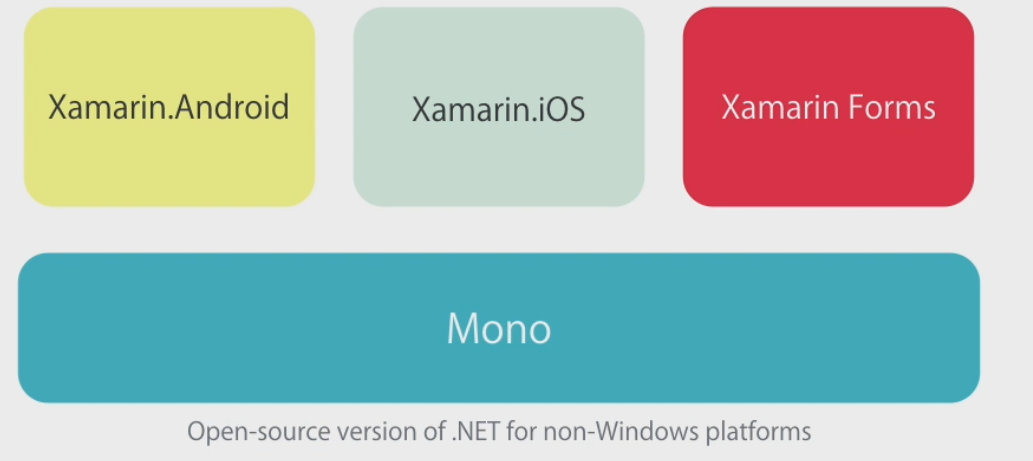
\includegraphics[width=0.7\textwidth]{arch-xamarin}
    \caption{Architecture Xamarin}
    \label{bat}
\end{figure}

 \vspace{0.5cm}
 
Tout d’abord, il y a l’approche native cette approche et plus souvent choisie si l’application comprends de nombreuses fonctionnalités spécifiques et composants personnalisés. Celle-ci se base sur Mono et ses 2 librairies Xamarin.Android et Xamarin.iOS.

 \vspace{0.5cm}
 
Puis, il existe l'approche avec xamarin.Forms permettant la mutualisation des interfaces.


\paragraph{L’approche native}
Afin de permettre le développement d’application mobile aux critères spécifiques, l’approche native permet au développeur de coder directement les interfaces en Natif.
Pour ce faire Mono bénéficie de 2 librairies couvrant 100\% des API Android et IOS soit:

\begin{itemize}
\item Mono for Android renommé en Xamarin.Android
\item MonoTouch renommé en  Xamarin.IOS
\end{itemize}

\begin{figure}[h]
    \centering
    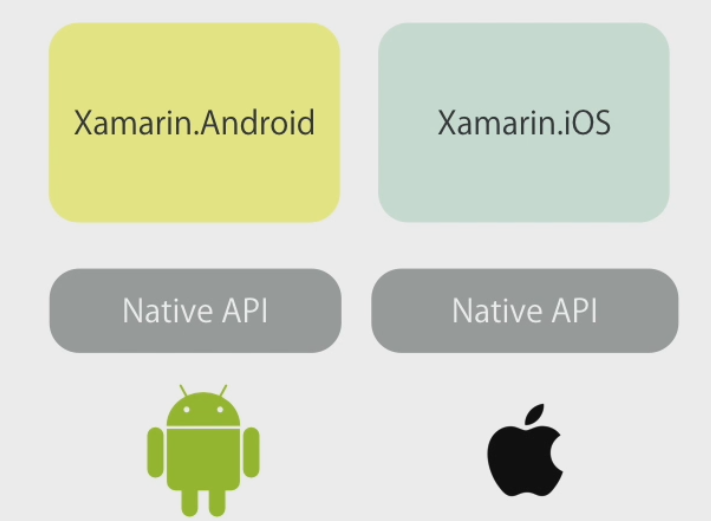
\includegraphics[width=0.5\textwidth]{lib-mono}
    \caption{Librairies Mono}
    \label{bat}
\end{figure}


 \vspace{0.5cm}
 
Ces bibliothèque donnent accès à la bibliothèque standard du framework .NET ainsi qu’aux APIs natives des plateformes visées par les bibliothèques ou les assemblies et namespaces correspondent aux classes en Objective-C ou JAVA.
 
 \vspace{0.5cm}
 
Ainsi, travailler sur ces classes revient comme à utiliser celle de la bibliothèque standard du framework .NET car ces libraires vont à l’intérieur appeler l’API correspondante.


\paragraph{L’approche xamarin.Forms}
Construite au-dessus des deux bibliothèques Xamarin.Android et Xamarin.iOS, Xamarin Forms est la librairie permettant la création d’interfaces unifiées aux différentes plateformes.

\begin{figure}[h]
    \centering
    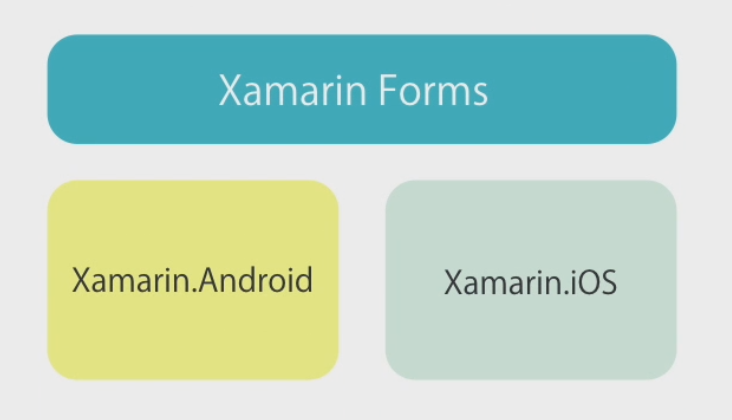
\includegraphics[width=0.5\textwidth]{lib-xamforms}
    \caption{Librairie Xamarin Forms}
    \label{bat}
\end{figure}

 \vspace{0.5cm}
 
Cela est rendu possible grâce à l’assembly nommé Xamarin.Forms.Core ainsi que les différentes  classes composant  Xamarin Forms ce qui permet de définir une API unique fonctionnant sur les trois plateformes afin de créer les interfaces utilisateurs.

 \vspace{0.5cm}
 
Xamarin Forms fonctionne en mappant les éléments correspondant à leur équivalent natif ce qui va rendre les applications complètement natives et va donc avoir le rendu natif sur chacune des plateformes.
 
 \vspace{0.5cm}
 
Ainsi Xamarin Froms permet l'écriture d’interface utilisateurs génériques quel que soit les plateformes. De surcroît cette librairie permet d’écrire du code spécifique à une plateforme en utilisant l’API exposé par chacune des libraires (Xamarin.Android, Xamarin.IOS) de manière à pouvoir ajouter/modifier les fonctionnalités les concernant.
 
 \vspace{0.5cm}
 
Par conséquent, nous avons donc d’un côté la possibilité d'écrire des interfaces génériques quel que soit les plateforme et d’un autre la capacité de personnaliser les différents éléments natif par le biais par exemple d’un renderer (rendu) côté natif.


\subsection{La compilation}

Afin qu’une application fonctionne sur la plateforme voulue il faut compiler celle-ci afin que la plateforme puisse la lire et l'exécuter.
 
 \vspace{0.5cm}
 
Nous allons voir ci-dessous les différentes stratégies de compilation mises en oeuvre en fonction de plateforme ciblée.

\subsubsection{La compilation sous Windows}

Le code C # est compilé en IL puis exécuté par le runtime, l’avantage de celui-ci est qu’il ne nécessite pas d'outils Xamarin c’est donc la solution la plus directe.

\subsubsection{La compilation sous Android}
Xamarin sous Android utilise une compilation divisée en deux phases (voir figure 12), la compilation en langage intermédiaire puis la compilation Just-In-Time (JIT).


\begin{figure}[h]
    \centering
    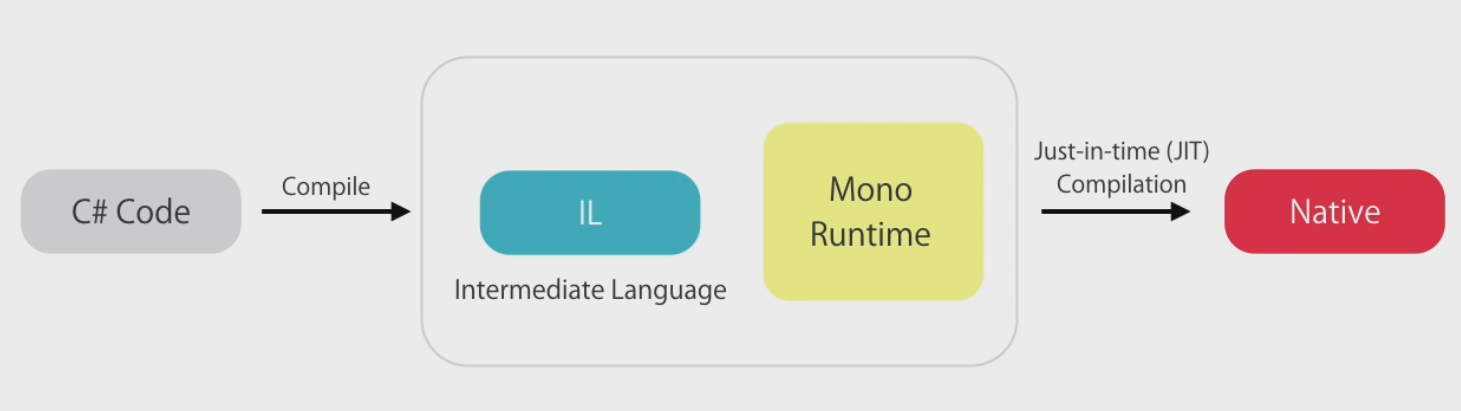
\includegraphics[width=0.9\textwidth]{compilation1}
    \caption{La compilation sous Android}
    \label{bat}
\end{figure}



 \vspace{0.5cm}
 
Lors de la première étape le compiler Xamarin C\# compile le code en langage intermédiaire (IL) et y intègre le runtime Mono (similaire au CLR) dans un package.
 
 \vspace{0.5cm}
 
Ensuite, quand l’application android est lancée le runtime se charge en mémoire et récupère le code IL puis compile celui-ci en code natif pour android.

\subsubsection{La compilation sous iOS}

Pour  la compilation sous iOS, le code C\# est compilé à l’avance la stratégie de compilation est donc ahead-of-time (AOT). Cette solution est due à la limitation qu’impose Apple, car celle-ci ne permet pas la génération de code d’exécution sur iOS.

\begin{figure}[h]
    \centering
    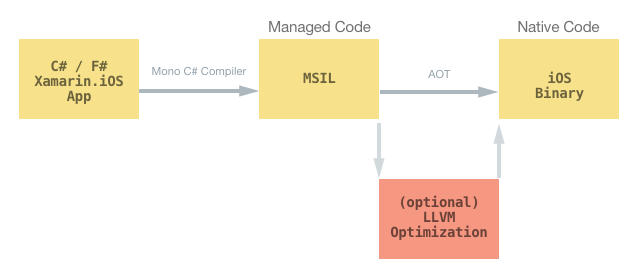
\includegraphics[width=0.9\textwidth]{compilation2}
    \caption{La compilation sous iOS}
    \label{bat}
\end{figure}



\newpage
\thispagestyle{empty}
\strut



\newpage
\setcounter{page}{24}
\begin{center}
\part{Processus étudié}
\noindent\rule{12cm}{0.4pt}
\end{center}
\setcounter{section}{0}

Le choix de la stratégie technologique d’une entreprise a un impact décisif sur son évolution, son organisation, sa pérennité. Par conséquent il crucial pour les entreprises de définir les meilleurs outils, technologies à employer afin d’en tirer le meilleurs avantage concurrentiel, la plus grande rentabilité en fonction de leur capacité interne ainsi que de leur capacité d’évolution.

 \vspace{0.5cm}
 
Par conséquent, il est nécessaire de déterminer d’une part si la technologie Xamarin dans son écosystème Microsoft bénéfice des qualités nécessaires pour le développement d’applications mobiles, d’autre part si cette solution proposée est suffisamment mature pour que des entreprises puisse l’employer de manière pérenne et dans quelles conditions.
 
 \vspace{0.5cm}
 
Dans cette optique, ce mémoire aborde tout d’abord les performances et le rendu de l’UI vis-à-vis du développement pur natif; l’écosystème Microsoft sera ensuite étudié afin de déterminer ses avantages et inconvénients; puis la maturité de la technologie sera mise en lumière; enfin nous situeront Xamarin face au marché des applications mobiles.

 \vspace{0.5cm}
 

 \section{Les performances de Xamarin}
 
 L’une des prérogatives affirmé par Xamarin concerne ses performances dites comme proches de celles du natif.
 
  \vspace{0.5cm}
 
Si cette affirmation se justifierait, Xamarin serait effectivement une solution viable concernant l’axe des performances et de surcroît cette technologie se distinguerait des solutions Hybrides.
 
  \vspace{0.5cm}
 
Toutefois, quand bien même Xamarin aurait des performances similaire au natif il est important de voir les aspects garantissant ces performances et quels sont leurs coûts.
 
  \vspace{0.5cm}
 
Ainsi, nous allons premièrement aborder le comparatif des performances entre le Natif, l’hybride et Xamarin; puis nous verrons les différentes techniques permettant à Xamarin d’optimiser ses performances; enfin nous conclurons sur les avantages et inconvénients liés aux performances. 

  \subsection{Les performances de Xamarin vis-à-vis du Natif et de l’Hybride}
 
 Dans un écrit à l’«International Conference on Mobile Services» nommé «A Quantitative Assessment of Performance in Mobile App Development Tools» un comparatif de performances concernant le Natif, l’hybride avec PhoneGap et Xamarin a été effectué.
 
 
   \vspace{0.5cm}
   
   
Pour chaque résultat de test effectué dans ce comparatif, celui-ci est la moyenne du même test effectué 5 fois et ce afin de bénéficier de la valeur la plus juste qui soit. 

   \vspace{0.5cm}
   
Nous utiliserons ci-dessous les résultats des performances obtenus par ce comparatif.

   \subsubsection{La performance au lancement de l’application}
   
 Le temps de lancement d’une application mobile est un facteur déterminant dans l’expérience utilisateur, car si celui-ci est trop long, l’utilisateur pourrait abandonner l’usage de l’application et se tourner vers un concurrent.
 
   \vspace{0.5cm}
   
Dans la figure ci-dessous, nous remarquons que sous Android le temps de lancement pour Xamarin est un peu plus rapide que l’hybride, cependant sous iOS Xamarin bénéficie d’un temps de lancement proche du natif et au moins 2 fois plus rapide que PhoneGap.

 \begin{figure}[h]
    \centering
    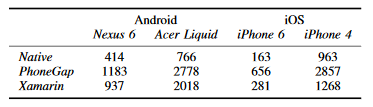
\includegraphics[width=0.7\textwidth]{a1}
    \caption{Performance au lancement de l’application (en millisecondes)
}
    \label{bat}
\end{figure}
 
    \subsubsection{La performance à la pause et à la reprise}
   
Concernant les changements d’état de l’application lorsque celle-ci est en pause puis reprends son activité nous remarquons que quelque soit la solution employée les performances sont extrêmement proches.

 \begin{figure}[h]
    \centering
    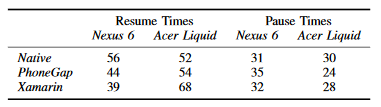
\includegraphics[width=0.7\textwidth]{a2}
    \caption{La performance à la pause et à la reprise (en millisecondes)}
    \label{bat}
\end{figure}
 
     \subsubsection{La performance à l’ouverture d’une nouvelle page}
   
Concernant les changements d’état de l’application lorsque celle-ci est en pause puis reprends son activité nous remarquons que quel que soit la solution employée les performances sont extrêmement proches.

 \begin{figure}[h]
    \centering
    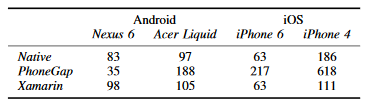
\includegraphics[width=0.7\textwidth]{a3}
    \caption{La performance à L’ouverture d’une nouvelle page (en millisecondes)}
    \label{bat}
\end{figure}
 
 \vspace{0.5cm}
  \vspace{0.5cm}

 
      \subsubsection{Le taux d’utilisation du CPU}
   
L’utilisation du CPU d’un mobile est directement lié à la consommation énergétique et donc à la durée d’une batterie. Il est par conséquent important qu’une application ne consomme pas déraisonnablement les ressources du CPU. Dans le comparatif, nous remarquons que le natif bénéficie d’excellentes performances et que PhoneGap ainsi que Xamarin consomment en moyenne plus de deux fois plus, avec cependant un léger avantage côté Xamarin.

 \begin{figure}[h]
    \centering
    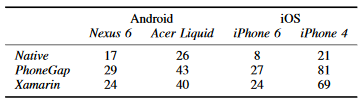
\includegraphics[width=0.7\textwidth]{a4}
    \caption{Le taux d’utilisation du CPU (en \%)}
    \label{bat}
\end{figure}
 
 \subsubsection{La taille de l’application}
   
La taille de l’application Xamarin sous sa forme d’APK pour Android sera conséquente car le package contient les éléments de Mono.Android ainsi nous avons ici 9,69MB soit environ neuf plus que le natif et plus de deux fois que l’hybride, cette taille est optimisable en utilisant la fonctionnalité Linker.

 \vspace{0.5cm}

Dans un second temps la taille de l'application Xamarin sous sa forme IPA pour iOS est ici de 2.7MB comparé à 0.62MB en natif et 7.4MB en hybride. Par conséquent, la taille de l’application en Xamarin est plus lourde qu’en natif car nous sommes obligés de prendre en compte le framework Mono ce qui alourdit le package de l’application.



 \begin{figure}[h]
    \centering
    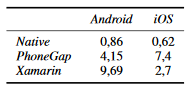
\includegraphics[width=0.334\textwidth]{a6}
    \caption{La taille de l’APK et IPA de l’application (en MB)}
    \label{bat}
\end{figure}
 
 
\subsubsection{La consommation en mémoire de l’application}
   
Pour une application limiter la consommation de la mémoire vive est un facteur important car si la mémoire vive est surchargée les performances du mobile s’en trouveront amoindries. Dans le test de la figure ci-dessous nous remarquons que la mémoire consommé par Xamarin et le Natif sont proches tandis que l’hybride PhoneGap sera plus vorace.


 \begin{figure}[h]
    \centering
    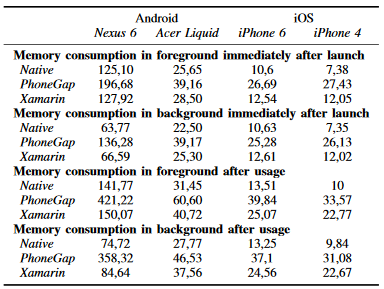
\includegraphics[width=0.7\textwidth]{a5}
    \caption{La consommation en mémoire de l’application (en MB)}
    \label{bat}
\end{figure}
 
 


\subsection{L’optimisation des performances en Xamarin}
 
Xamarin met à disposition de nombreuses techniques, méthodes et outils permettant l’optimisation des performances d’une application mobile. Ainsi la réalisation d’une application performante va aussi reposer sur la capacité des développeurs à mettre en oeuvre ces techniques et bonnes pratiques. 
  
   \vspace{0.5cm}
   
Nous allons voir ci-dessous solutions techniques générales afin d’optimiser au maximum les performances d’une application mobile Xamarin.


 \subsubsection{Monitorer son application et déceler les optimisations grâce à Xamarin Profiler}
 
Xamarin Profiler est un outil à destination de Xamarin.iOS et Xamarin.Android permettant de suivre l’utilisation de la mémoire d’une application mobile, d’enregistrer les temps de fonctionnement des méthodes de l’application et ce afin de déterminer les coûts d'exécution du code dans l’objectif de proposer aux développeurs les solutions d’optimisations les plus pertinentes.

\vspace{0.5cm}
   
Par conséquent cet outil permettra aux développeurs de trouver les différents problèmes liés aux performances dans une application mobile android ou iOS. Cela est un énorme avantage tant les problématiques en termes de performances dans l’utilisation des solutions cross-plateformes peuvent impacter la décision du choix technologique pour le développement d’une application.
 
 
 \subsubsection{La libération de la mémoire pour les ressources non gérés grâce à l’interface IDisposable}
 
 L’interface IDisposable, fournit un mécanisme permettant la libération des ressources non gérées qui peuvent inclure des fichiers, des flux ou encore des connexions réseau.
 
\vspace{0.5cm}
   
Dans l’exemple de la figure ci-dessous, un fichier texte est lu jusqu’à la fin de celui-ci grâce à la méthode “ReadToEnd()”, si une exception se produit dans le bloc try, la méthode Dispose() définie dans l’interface IDisposable sera appelée et par conséquent la ressource sera gérée et libère la ressource; dans le cas contraire sans utiliser cette méthode et si une exception se produit la ressource deviendra une ressource non gérée et dès lors engendrant des effets de bords.

 
 \begin{figure}[h]
    \centering
    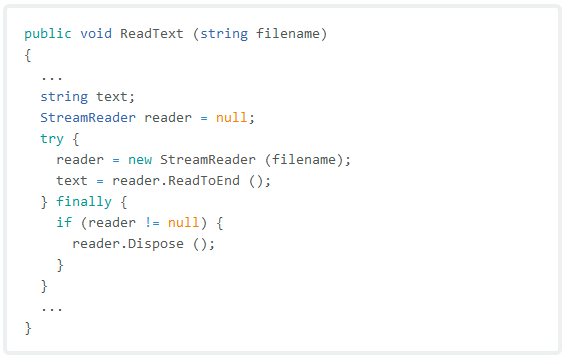
\includegraphics[width=0.7\textwidth]{b1}
    \caption{IDisposable}
    \label{bat}
\end{figure}
 
 Ainsi, par l’utilisation de cette interface IDisposable celle-ci réduira les effets de bords d’une application mobile et pourra donc être à l’utilisation plus légère en mémoire, moins consommatrice en data et en batterie.
 
\subsubsection{Le désabonnement des événements afin d’éviter les fuites mémoires}
  
 La gestion de l’abonnement et du désabonnement aux événements doit être pris en compte afin d’éviter les fuites de mémoire. La prise en compte du désabonnement est simple à mettre en oeuvre, celui-ci doit être pris en compte avant qu’un objet contenant un abonnement ne soit supprimé. Afin de prendre en compte cette gestion du désabonnement la classe doit implémenter l’interface IDisposable afin de définir la méthode Dispose qui contiendra le désabonnement à l'événement ciblé.
 
 
\subsubsection{L’utilisation des références faibles afin de se prémunir des objets immortels}
  
Il est important dans le développement d’une application mobile de ne pas faire de références fortes circulaires, car dans le cas ou deux objets bénéficie de références fortes l’un vers l’autre ceux-ci deviennent immortels et ne pourront pas être supprimés par le garbage collector même s'ils ne sont plus employés, en conséquence l’application sera plus lourde en mémoire à l’utilisation. 
La solution pour éviter ce problème est de remplacer les références fortes par des références faibles. Une référence faible va faire référence à un objet tout en autorisant cet objet d’être récupéré par le garbage collector. En C#, une référence faible est créée par le type WeakReference, l’objectif ici est de transformer dans les références fortes circulaires, une référence forte en une référence faible, afin que le garbage collector puisse faire son travail.

\subsubsection{Reporter le coût de la création des objets avec l’initialisation “Lazy” }
  
L’initialisation avec le type Lazy va permettre à un objet d’effectuer sa création uniquement lors de sa première utilisation. En définitive l’initialisation avec “Lazy” va permettre de réduire les besoins en mémoire ainsi que d’améliorer les performances de l’application.
 
\subsubsection{Utiliser des opérations asynchrones pour ne pas bloquer le thread UI}
  
Le framework .NET met à disposition les opérations asynchrones par l’intermédiaire des mots-clés await et async et Task.Run, leur objectif est de toujours laisser le thread UI débloqué afin que l’application ne freeze pas sur un processus et donc n’impacte pas l’expérience utilisateur.
 
\subsubsection{Utiliser le garbage collector SGen}
  
SGen est un garbage collector permettant de réduire le temps nécessaire dans l'exécution de ses tâches de récupération par conséquent cela va améliorer les performances de l’application.
 
\subsubsection{Réduire la taille de l’application avec Linker}
  
Linker est un outil de pour la compilation permettant grâce à une analyse de définir les méthodes et types utilisés par l’application et de retirer ceux qui ne serait pas utilisés. L’objectif ici est de réduire la taille finale de l’application. Car il est important de savoir que dans une application Xamarin le framework .NET est inclut d'où une taille d’application qui sera toujours plus grande qu’en natif, toutefois cette taille peut être limitée en utilisant l’option du Linker.
 
\subsubsection{Réduire la taille de l’application en ciblant l’architecture du processeur}

Une des forces de Xamarin est aussi de fournir pour les plateformes Android et iOS une version compilée de l’application ciblant chaque architecture réduisant ainsi la taille de l’application.

\subsubsection{Optimiser le chargement des images}

Les images sont des ressources qui ont un coût important pour l’application, afin de minimiser l’impact sur le CPU lors du chargement de celle-ci, il est nécessaire de définir les images dans différents formats de résolution en fonction de leur affichage.

\subsubsection{Limiter l’utilisation de la bande passante lors des communications avec les web services}

Afin de réduire l’utilisation de la bande passante dans une application Xamarin offre deux solutions. 
  
\vspace{0.5cm}
   
La première consiste à compresser les données à transférer, cependant cette solution sera consommatrice en batterie car utilisera le CPU pour effectuer cette opération.
  
\vspace{0.5cm}
   
La deuxième solution est d’utiliser le format JSON pour l'échange de données entre les web service lié avec l’utilisation de DTO (data transfer object), car celui-ci contient jeu de données. L’objectif ici est de limiter le nombre d’appels effectués aux webservices.

\subsection{Conclusion sur les performances}

Ainsi, Xamarin offre des performances similaires au natif ainsi que des performances meilleures que l’hybride. De plus, Xamarin permet d’aller plus loin en fournissant des outils tel que Linker afin d’optimiser son application mobile au maximum. Toutefois, cette optimisation des performances est dépendante de la connaissance et la formation des développeurs sur la technologie Xamarin. Ainsi ces notions complémentaires induisent une solution Xamarin plus riche mais aussi une courbe d’apprentissage des développeurs tirée vers le bas.


\section{L’écosystème Microsoft}

Microsoft bénéficie d’un large panel de solutions et d’outils permettant de faciliter et encadrer le développement d’applications mobiles. Ces solutions ont comme avantage d’être pensées afin qu’elles ne soient pas dépendantes les unes des autres mais qu’elles soient plus facilement adoptables qu’une autre solution tierce par exemple en permettant le téléchargement d’une base d’un projet serveur pour une application mobile. Par conséquent Microsoft pousse l’adoption de ses produits en réduisant le temps de développement pour les développeurs tout en leur fournissant une réponse adaptée à leurs besoins tout en ayant des coûts attractifs.
 
\subsection{Les outils de développements}

\subsubsection{Visual Studio}

Visual Studio est un Environnement de développement (IDE) comprenant un ensemble complet d’outils de développement. Depuis sa première version publiée en 1997 cet IDE a évolué et bénéficié de nombreuses mises à jours et versions jusqu’à acquérir aujourd’hui sa robustesse. Ainsi grâce à cet IDE nous pouvons développer de nombreux types d’application qu’elles soient à destination du Web, du Cloud ou encore du mobile, son objectif est de rendre possible la création d’applications quel que soit la plateforme visée.
  
\vspace{0.5cm}
    
Par conséquent, Visual Studio intègre Xamarin pour le développement d’application mobile. Ainsi nous retrouvons de nombreux outils afin de rendre le développement d’application plus souple et rapide.
   
\vspace{0.5cm}
   
Parmis ces outils nous retrouvons de manière non exhaustive :
   
  
\paragraph{Xamarin Inspector} 
Xamarin Inspector est un outil permettant le diagnostic et le prototypage de modification dans une application. L’inspecteur s’intègre au flux du debuging de l’IDE afin d’apporter une aide et diagnostique à l’application en exécution.

\paragraph{Xamarin profiler}
Cet outil a pour objectif de collecter les informations clés sur une application Xamarin. Ces informations seront utilisées afin de détecter les fuites de mémoire, les goulots d’étranglement dans l’objectif d’optimiser les performances de vos applications.

\paragraph{Forms previewer}
Afin de réduire le temps de Build and Run lors du développement d’une application, Forms previewer est outil dont l’objectif est d’afficher un aperçu en temps réel à coté du code d’une interface développée en XAML.

\paragraph{iOS simulator}
L’outil iOS simulator a pour objectif de fournir un iPhone virtuel testable directement sur son Mac.

\paragraph{Xamarin Live Player}
L’outil Xamarin Live Player va autoriser le développeur à associer un appareil Android ou iOS avec Visual Studio afin de bénéficier d’un mobile affichant en temps réel la version de l’application telle qu’elle est codée sur l’IDE.
   
\paragraph{Xamarin Test Recorder}
Cet outil a pour objectif d’étudier la manière dont les utilisateurs interagissent avec une application afin de créer des tests automatisés en fonctions des interactions répertoriées.

\paragraph{La personnalisation de l’IDE}
Visual Studio est un IDE très souple et entièrement personnalisable, couleurs, barre des tâches, raccourcis, emplacement des éléments tout y est conçu pour y être intuitif pour l’utilisateur afin que son IDE se conforme à son utilisation.

\paragraph{Intellisense}
Intellisense est un outil facilitant grandement la vie des utilisateurs de l’IDE car il permet l’auto-complétion par suggestion et sélection intuitive grâce à un système de filtre (pour les propriétés, événements, méthodes), la redirection vers les implémentations et définitions, en définitive c’est un outil qui a pour vocation à être utilisé au quotidien.
    
\paragraph{Les plugins}
Visual Studio bénéficie de nombreux plugins permettant d’accélérer le développement tel que codemaid permettant la simplification et l’épuration du code, ou encore ReSharper permettant entre autre la détection des erreurs de compilation, des redondances et odeurs de code.

\paragraph{Les package NuGet}
Les NuGets sont des bibliothèques externes, celles-ci sont directement accessibles par le développeur à l’interieur de Visual Studio afin d’ajouter une bibliothèque tel que par exemple Facebook iOS SDK permettant entre autre la gestion de la connexion à une application via Facebook.





\subsection{Le Cloud Microsoft Azure}
Azure propose de nombreux services Cloud PaaS (Platform as a Service) permettant d’héberger les fonctionnalités nécessaires à une application mobile, fournir des outils de DevOps ainsi que de proposer un outil de collaboration. Les avantages à utiliser les services du cloud sont multiples tel que la réduction des coûts des services employés car la facturation s’effectue progressivement à la consommation, la qualité du service proposé, la rapidité de mise en place des solutions proposés grâce aux nombreuses documentations et projets types téléchargeables, diminuer en complexité. 
      
\vspace{0.5cm}
   
Ainsi nous allons voir ci-dessous les différents outils communéments utilisés lors du développement d’une application mobile en utilisant les services du cloud.


\subsubsection{Les services d'application mobile}
Les services proposés par le cloud Azure à destination des applications mobiles sont principalement orientés pour l’enregistrement des données dans le cloud, l’authentification des utilisateurs ainsi que l’utilisation d’un système de Push notification centralisée.
 
\paragraph{L’enregistrement des données dans le Cloud}
Azure propose plusieurs services de stockage de données en fonction de leur type et des besoins de l’application. Ainsi pour le stockage de données relationnelles on privilégiera un serveur SQL et pour des fichiers multimédias on utilisera un blob storage. 
De plus, Azure permet par l’intermédiaire de Mobile Apps de fournir des fonctionnalités permettant la synchronisation des données avec les applications Windows, iOS, Android permettant l’interaction avec les données même en étant hors connexion.

\paragraph{L’authentification des utilisateurs}
Azure propose un système d’authentification d’utilisateur pour les applications mobiles prenant en charge pas moins de cinq fournisseurs d’identité tels que Google, Facebook, Twitter,  Microsoft et Azure Active Directory.
 
\paragraph{Azure Notification Hubs}
Azure Notification Hubs, propose une solution clé en main, permettant d’envoyer facilement des notifications push à partir de n'importe quel backend sur les plateformes Windows, Android et iOS.
Ce service permet de gérer efficacement les notifications personnalisées et cibler son audience et utilisateurs souhaités tout en prenant en considération des appareils utilisés.

\subsubsection{Les services permettant d’assurer la qualité de l’application}
Afin de garantir une application mobile éprouvée et robuste, Azure met à disposition deux services de suivi qualité et de testing, ces services sont xamarin test cloud et Hockey App.
 
\paragraph{Xamarin test cloud}
L’une des complexités du développement mobile cross-plateforme est que l’application résultant sera utilisé sur une pléthore d’appareil. De ce fait il devient très complexe de tester son application et d’être sur des résultats obtenus car chaque périphérique (smartphone, tablette ... ) bénéficie de ses propres caractéristiques matérielles et logicielles.
      
\vspace{0.5cm}
   
Pour palier à cela Xamarin test cloud propose un service permettant d’organiser des tests automatisés sur ses propres applications pour plus de 2000 périphériques différents.
Grâce à ce service des rapports détaillés des tests passés sur les applications permettent de définir les problèmes potentiels et à corriger.
Ainsi grâce à ce service il devient possible de déployer sur les stores des applications déjà éprouvés de multiples batteries de tests garantissant la qualité de l’application.

\paragraph{Hockey App}
Hockey App est un puissant outil ayant pour rôle sur une application donnée de monitorer, générer et récupérer des analytics et métriques concernant les rapports d’erreurs, feedbacks et comportement utilisateurs sur les devices qu’ils utilisent.
L’intérêt d’Hockey App est de bénéficier d’un retour utilisateur grâce à de nombreux résultats et commentaire afin de corriger les différents problèmes pouvant survenir ainsi que d’orienter le développement de l’application pour une meilleure expérience utilisateur.
 
 \subsubsection{Visual Studio Team Services}  
VSTS ou Visual Studio Team Services est un outil de collaboration comprenant un ensemble d’outils pour le développement logiciel. Basé sur le Cloud, VSTS est une solution complète qui incorpore principalement : 

 \begin{itemize}
\item le contrôle de version centralisé par Team Foundation Version Control ou Git
\item le suivi des tâches par la gestion de portefeuille agile et tableaux de tâches
\item l’intégration et déploiement en continue via le cloud
\end{itemize}
     
\vspace{0.5cm}
   
VSTS fonctionne de concert avec Visual Studio ce qui permet au développeur de travailler en équipe de manière efficace et dynamique sur un même projet.

 
 \subsection{Conclusion sur l'écosystème Microsoft}
 Microsoft nous propose par le biais de Visual Studio d’un large panel de fonctionnalités permettant au développeur de se concentrer sur l’essentiel, le développement de l’application. Ces fonctionnalités telles que Xamarin Live Player qui octroie la capacité de tester en temps réel le code que l’on développe vont lever de nombreuses barrières pour le développeur le faisant économiser du temps et améliorant sa productivité.
D’autre part, Visual Studio couplé aux services proposés par le cloud Microsoft Azure fera bénéficier au équipes de développement de solutions prêtes à l’emploi et facilement intégrables à leur projets ainsi que des solutions de monitoring et de tests.
     
\vspace{0.5cm}
   
Finalement, les nombreuses solutions et outils proposées par Microsoft permettent aux entreprises le développement d’applications mobiles performantes et de qualité tout en leur facilitant leur travail dans la conception et le suivi. Toutefois, l’apprivoisement de ces nombreux outils risque de constituer un coût en formation ainsi qu’en temps d’adoption pour les entreprises, car il n’est pas aisé de prendre en mains rapidement tous ces outils qui requièrent souvent un changement d’habitude de travail ainsi qu’un temps de configuration.

 
 
 
 \section{Xamarin, une technologie dynamique et mature}
L'un des facteur d'adoption d'une technologie est lié à son dynamisme et à sa maturité.
      
\vspace{0.5cm}
   
Dépendant des ces facteurs une technologie pour qu'elle soit adoptée doit :

\begin{itemize}
\item Se populariser par l’intermédiaire des entreprises qui vont l’utiliser, l’améliorer, mais aussi au travers de la communauté et des portes paroles, étendard crédibles qui croient en elle et qui vont participer à sa diffusion et évolution.
\item Avoir une bonne expérience technique de son milieu
\item Profiter d’une évolution éclairée
\end{itemize}
 
 
\vspace{0.5cm}
   
De ce fait, pour vérifier si Xamarin est une technologie dynamique et mature nous allons voir l’évolution historique de la technologie, son dynamisme, sa richesse documentaire et enfin son support réactif.

\subsection{L’évolution de Xamarin de 2001 à nos jours}
 
 L’histoire de Xamarin commence en 1999 ou Miguel de Icaza et Nat Friedman fondent Ximian. Ces deux anciens stagiaires de Microsoft vont se consacrer à étudier la possibilité d’implémenter la Common Language Infrastructure (CLI) de la plateforme .NET pour Linux ce qui aboutira au lancement du projet open source Mono en 2001.
      
\vspace{0.5cm}
   
Ensuite, en 2003 Novell rachète Ximian ce qui va accélérer le développement de Mono jusqu’à la sortie de sa version 1.0 le 30 juin 2004.
     
\vspace{0.5cm}
   
Par la suite en septembre 2009 le support pour iOS est publié sous le nom de Mono Touch, la version de Mono pour Android soit Mono for Android 1.0 ne sera lui publié qu’en 2011. A partir de cet instant il devient possible de réaliser des applications natives pour ces plateformes en utilisant Visual Studio, le framework .NET et le C#.
      
\vspace{0.5cm}
   
En Avril 2011 la société spécialisée dans l’émulation de terminaux Attachmate achète Novell et licencie massivement les employés de Novell remettant ainsi en question la pérennité de Mono.
      
\vspace{0.5cm}
   
Puis, le 16 mai 2011 Miguel de Icaza annonce que Mono serait soutenu et développé par la nouvelle entreprise Xamarin, l’équipe Mono va se reformer et intégrer Xamarin. En Juillet 2011 la filiale de Attachmate Novell accorde une licence perpétuelle de Mono à Xamarin.
      
\vspace{0.5cm}
   
A partir de cet instant Xamarin va cumuler les levées de fonds jusqu’à atteindre 82 millions de dollars ainsi que de nombreuses innovations tel que par le biais d’un IDE complet avec Xamarin Studio (anciennement MonoDevelop).
      
\vspace{0.5cm}
   
Enfin, le 24 février 2016 Xamarin est acquis par Microsoft. Par cette acquisition Microsoft va dans un premier temps stabiliser la technologie puis ouvrir ses portes à Xamarin afin de mettre en synergie ses différentes équipes tel qu’avec le Cloud Azure ou les spécialistes Xamarin ont guidé les équipes d’Azure pour la mise au point des nombreux services pour la gestion des back-end des applications Android et iOS.
L’objectif de Microsoft est clairement de fournir une solution adaptée aux problématiques du développement mobile tout en mettant en avant les services Cloud.
      
\vspace{0.5cm}
   
Peu de temps après son acquisition Microsoft a fait le choix de rendre open source Mono ainsi que de rendre son utilisation gratuite.
A l’instant où Mono est passé sous licence MIT cela a permis à d’autres sociétés de contribuer et apporter de nouvelles fonctionnalités dans l’écosystème .NET. C’est le cas de Samsung qui a collaboré avec Microsoft afin de porter le framework .NET sur le système d’exploitation open source Tizen, OS utilisé entre autre sur les montres connectés Gear 2 de Samsung. Ce portage a abouti à l’élaboration de Visual Studio Tools for Tizen permettant le développement d’application mobile avec Xamarin Forms. De ce fait la stratégie de microsoft est axée sur la popularisation de l’outil, l’écoute de la communauté et l’amélioration continue de ses technologies.   
      
\vspace{0.5cm}
 
 En ayant acquis Xamarin, Microsoft grâce à son envergure permet à cette technologie de bénéficier d’un cadre solide et durable assurant la pérennité de celle-ci. 


 \subsection{Le dynamisme de la technologie}
 
 La communauté de Xamarin est très active d’une part grâce aux nombreux partenaires tel que Coca Cola, Hp ou encore Samsung comme vu précédemment avec son portage du framework .NET sur Tizen; d’autre part grâce à la communauté très présente sur les forums tel que sur «https://forums.xamarin.com/»  ou des centaines de milliers de posts ont été effectués et ce rigoureusement catégorisé, ainsi que sur github ou la technologie évolue de manière très régulière tel que avec Xamarin.Forms disponible sur le dépôt suivant «https://github.com/xamarin/Xamarin.Forms».


 \subsection{La richesse documentaire}
 Un des facteurs d'adoption de la technologie Xamarin est due à sa richesse documentaire et ses nombreuses formations.
  
\vspace{0.5cm}
   
Tout d’abord, nous avons les Xamarin Workbooks, ces documentations et guides sont idéal pour l’apprentissage et l’expérimentation car ils bénéficient de nombreux exemples de code et aides pédagogiques.
  
\vspace{0.5cm}
   
Puis nous avons Xamarin University où sont dispensés des formations sur le développement d’application mobiles par l’intermédiaire d’experts mobiles. La formation par la Xamarin University a aussi pour objectif de certifier les participants leur permettant de bénéficier d’une qualification qui est une aide précieuse pour la recherche d’un emploi dans ce domaine.



 \subsection{Xamarin, un support toujours à jour}
 L’une des grandes forces de Xamarin est qu’elle offre le support d’iOS le même jour de la sortie d’une nouvelle version, cela a été le cas pour les version d’iOS 5, 6, 7, 8, 9 et 10. Une telle prouesse est rendue possible grâce à la prise en compte des versions Beta d’iOS.
  
\vspace{0.5cm}
   
Pour Android la stratégie est différente car le taux d’adoption des nouvelles versions est nettement plus faible que celles d’iOS par conséquent le support ne s’effectue pas le même jour mais est tout de même prise en charge rapidement.

\subsection{Conclusion sur le dynamisme et la maturité de Xamarin}
Xamarin c’est ouvert au monde depuis son rachat par Microsoft en proposant une solution de développement d’application mobile devenue gratuite ainsi que sa mise à disposition en open source. Grâce à cela de plus en plus de personnes se tournent vers cette technologie et grâce au cadre mis en place par Microsoft la communauté peut clairement s’exprimer par l’intermédiaire de son forum ainsi que se former grâce aux outils mis à disposition. De plus Xamarin prouve aussi son dynamisme par l’évolution des différents Git démontrant que la technologie ne cesse de progresser, ainsi que par son support des nouvelles versions iOS le jour même de sa sortie. Xamarin bénéficie donc d’un cadre dynamique mais prouve sa maturité en étant soutenu et utilisés par de grands groupes ainsi qu’en ayant toujours réussi à aller de l’avant depuis son commencement historique en 1999.
 
 \section{Xamarin face au marché des applications mobiles}
 
Nous avons vu précédemment qu’il existe de nombreuses solutions technologiques dans le développement d’application mobiles que ce soit par l’intermédiaire du natif, de l’hybride ou encore du cross-plateforme natif.
  
\vspace{0.5cm}
   
Dans cette section nous allons voir quel est l’avantage concurrentiel de Xamarin qui pousserait son adoption par les entreprises d’un point de vue des ressources internes à l'entreprise, de l’organisation des équipes et des coûts qui en découlent.

  \subsection{Une réduction du nombre d’équipes et d’intervenants aux projets}
Une force de la technologie cross plateforme Xamarin impactant la composition et la logique de gestion et d'interaction des équipes de développement est sa capacité à casser l’approche de l’architecture en silo du développement natif (voir figure ci-dessous).
 
 \begin{figure}[h]
    \centering
    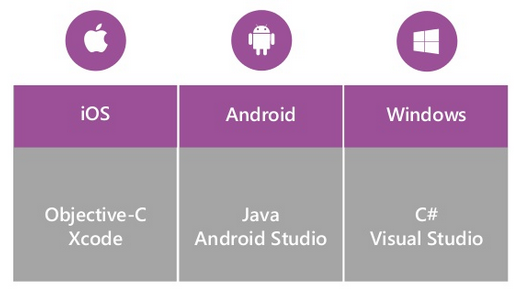
\includegraphics[width=0.8\textwidth]{c1}
    \caption{Architecture en silo}
    \label{bat}
\end{figure}
 
 
 En effet, lorsque les entreprises s’orientent sur le choix du développement natif d’une application mobile elles vont être contraintes à utiliser l’approche de l’architecture en silo. Cette approche a pour conséquence de multiplier les technologies, les langages et les outils utilisés.
C’est à dire qu’il n’y aura pas de code partagé entre les différentes plateformes, on utilisera des langages différents tel que :
\begin{itemize}
\item Objective-C ou Swift pour iOS
\item Java pour Android
\item C\# pour Windows
\end{itemize}
  
\vspace{0.5cm}

 
 
 
De plus, pour développer sous chaque OS on sera obligé de bénéficier d’un environnement de développement différent tel que :
\begin{itemize}
\item Xcode pour iOS
\item Android Studio pour Android
\item Visual Studio pour Windows
\end{itemize}
   
\vspace{0.5cm}

Cette multitude de technologies et d’outils à gérer va induire, pour mener son projet à bien, la constitution dans la majorité des cas d’une équipe de développement par plateforme comprenant des intervenants bénéficiant de compétences distinctes sur chaque plateforme.
    
\vspace{0.5cm}

De ce fait, en utilisant cette approche d’organisation pour le développement d’un projet d’application mobile sur les plateformes Android, iOS et Windows va aboutir à la création de trois équipes multipliant au minimum par trois les efforts nécessaires. 
    
 
\vspace{0.5cm}

Cette multiplication est due aux impératif propres à chaque équipe car il faudra que les besoins du projet soient bien compris, qu’ils soient en adéquations avec les autres équipes dans l’évolution de l’application ce qui va engendrer de multiples intermédiaires par le biais de réunions et ajustements puisque chaque équipe ne bénéficiera que de la vision propre à son projet.
    
\vspace{0.5cm}

Néanmoins, cette approche de développement en natif peut être optimisée en employant la méthode du Lean. Cette méthode a pour objectif d’optimiser les cycles de projet en incluant les acteurs de la création de l’application dans différentes les étapes de la conception de l’application. Cette vision d’organisation aura pour conséquence la formation d’une équipe pluridisciplinaire ayant une capacité de travail leur permettant d’avancer conjointement avec les différentes applications à développer sur les plateformes ciblées. Les coûts et les délais induits par les différentes interactions sont par conséquent réduits, cependant d’un point de vue recrutement, le personnel étant plus compétent et souple celui-ci bénéficiera d’un salaire plus élevé mais le nombre du personnel sera revu à la baisse.
    
 \vspace{0.5cm}

A contrario, Xamarin propose de casser les silos en autorisant le développement de manière simultanée d’une application mobile à destination de plusieurs plateformes. Grâce à son architecture une équipe projet unique pourra comme en développement hybride s’assurer du développement de l’application. 
 \vspace{0.5cm}

Les avantages de l’organisation en une équipe unique par projet de développement mobile en utilisant une technologie unique sont nombreux. Tout d’abord, les développeurs ont un environnement de travail harmonisé exploitant chacun les mêmes technologies et outils, supprimant de cette façon la barrière des connaissances disparates entre les différents interlocuteurs. Ensuite, la progression et la communication sur l’avancée du développement sur les plateformes est unifiée. De ce fait outre le gage de qualité pour un client bénéficiant d’une avancée claire et constante sur son projet, les interactions et communication avec les multiples parties prenantes seront réduites à l’essentiel pour plus de productivité. De plus, la constitution d’une équipe unique à pour conséquence de diminuer le nombre d’intervenants sur un projet de développement mobile donc de diminuer drastiquement les coûts de production. Enfin, grâce à son architecture, la maintenance applicative devient très aisée et l’intégration de nouvelles fonctionnalités et correctifs s’effectuent aisément, ce qui est un facteur important dans la diminution des coûts donnant ainsi un avantage concurrentiel aux entreprises l’utilisant.

\subsection{Le recrutement et l’engouement envers Xamarin}
Xamarin depuis son rachat et sa mise à disposition gratuitement dans Visual Studio annoncé le 31 mars 2016 pendant la conférence Build 2016 de Microsoft suscite un engouement de plus en plus important auprès des développeurs. Cet engouement est visible grâce au statistiques issues du site Indeed visibles sur les figures ci-dessous, ou depuis l'événement de la Build 2016 de plus en plus de développeur cherchent un poste sur cette technologie. 

 \vspace{0.5cm}
 
A contrario, nous remarquons sur les technologies hybrides basée sur Cordova, que les développeurs délaissent de plus en plus PhoneGap au profil d’Ionic mais cet engouement envers cette technologie hybride ne constitue pas la moitié de celle accordée à Xamarin.

  \begin{figure}[h]
    \centering
    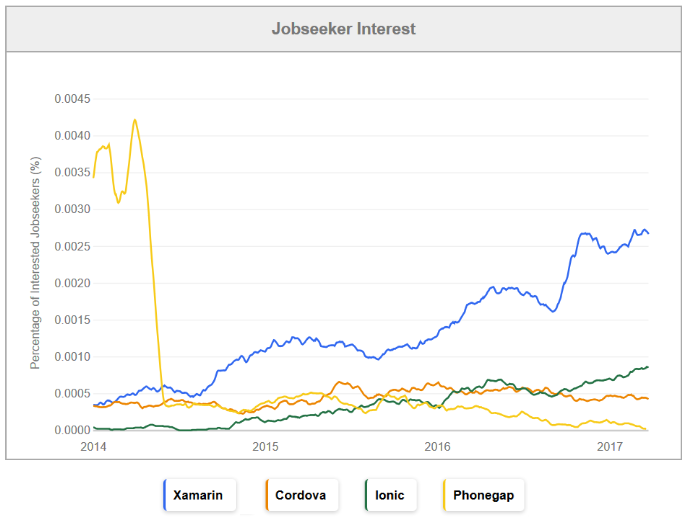
\includegraphics[width=0.6\textwidth]{f1}
    \caption{Courbe de l'intérêt des développeurs pour les offres d'emplois concernant Xamarin, Cordova, Ionic et Phonegap}
    \label{bat}
\end{figure}

 Néanmoins, si nous regardons ce phénomène vis-à-vis de l’intérêt porté par les développeurs sur les technologies natives celles-ci supplantent à l’heure de manière magistrale les technologies hybrides et cross-plateformes (voir la figure ci-dessous).
 
   \begin{figure}[h]
    \centering
    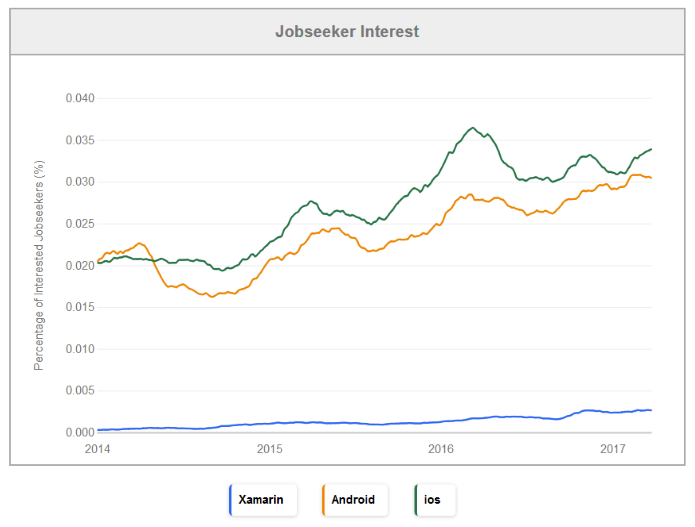
\includegraphics[width=0.6\textwidth]{f2}
    \caption{Courbe de l'intérêt des développeurs pour les offres d'emplois concernant Xamarin, Android et iOS}
    \label{bat}
\end{figure}

Un autre facteur à prendre en compte est l’émergence des entreprises voulant se spécialiser dans ces technologies innovantes et les entreprises ouvrant des postes sur ces technologies. Nous remarquons dans la figure ci-dessous, que les offres d’emplois proposées sont bien inférieures aux nombre de développeurs disponibles. Cela est dû à plusieurs facteurs, premièrement, plus une technologie est nouvelle et prometteuse plus l’attrait des développeurs dans ce cas majoritairement non qualifiés sera important, car le métier de développeur implique à toujours se former tout au long de sa vie et à se positionner sur les technologies les plus prometteuses et pérennes afin de bénéficier des meilleures opportunités. Deuxièmement, les entreprises mettent beaucoup de temps avant de considérer les nouvelles technologies car cela implique des nombreux coûts ainsi que de transformer leur fonctionnement interne.

   \begin{figure}[h]
    \centering
    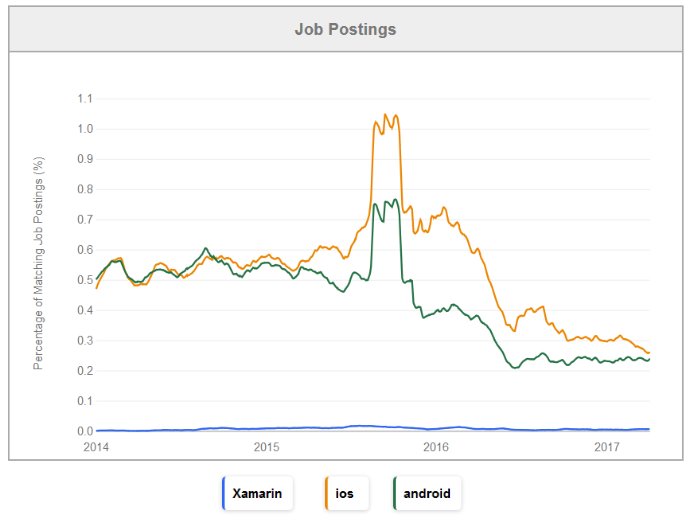
\includegraphics[width=0.8\textwidth]{f3}
    \caption{Courbe de l'évolution du nombre de postes proposé pour Xamarin, iOS et Android}
    \label{bat}
\end{figure}

 Par conséquent l’étape cruciale du recrutement de développeurs spécialisés et qualifiés devient ardue pour l’entreprise car les ressources alliant ces qualités sont limitées sur le marché et cette faible disponibilité va engendrer des coûts.
     
\vspace{0.5cm}

D’après les données du site de mise en relation Hired le tableau des rémunérations pour le développement en natif Android et iOS ainsi que pour les développeurs .NET sont les suivantes :

 
   \begin{figure}[h]
    \centering
    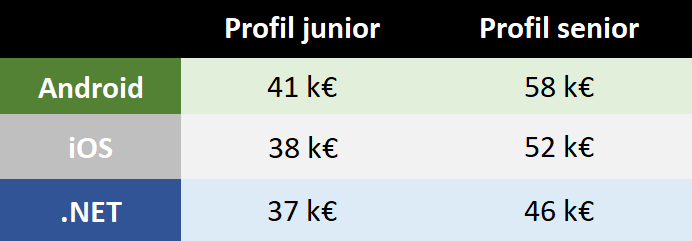
\includegraphics[width=0.6\textwidth]{f4}
    \caption{Tableau des rémunérations en fonction des plateformes de développement}
    \label{bat}
\end{figure}
 
 
On constate alors que les développeurs Android sont les plus coûteux suivis ensuite d’iOS et enfin les moins cher les développeurs .NET. Cependant les comparatifs de rémunération effectués vis-à-vis des technologies émergentes sont biaisées pour plusieures raisons. La première étant la faible disponibilité des développeurs qualifié sur ces technologies, deuxièmement un développeur .NET pour Xamarin doit bénéficier d’une expérience supplémentaire tel qu’une certification Xamarin. De ce fait les développeurs qualifiés en Xamarin seront difficiles à dénicher et de par leur positionnement bénéficieront d’une rémunération très attractive et bien supérieur au natif.

\subsection{La complexe formation en Xamarin}
Xamarin bénéficie d’un environnement riche avec une technologie complète ainsi que d’une multitude d’outils à maîtriser. Le corollaire de cela vis-à-vis de la formation est la difficulté à former rapidement tant la courbe d’apprentissage s’en trouve impactée et tirée vers le bas à cause d’un bagage technique trop important.
 
\subsection{Une offre tarifaire très concurrentielle}
 Depuis que Microsoft ait supprimé le système de licence payante en intégrant gratuitement Xamarin à Visual Studio cela autorise maintenant les développeurs à se former sur la technologie, la tester, voir sa viabilité ainsi que de rendre cette technologie plus populaire.
      
\vspace{0.5cm}

Par ailleurs Microsoft c’est orienté sur une stratégie marketing de type longue traîne, proposant ainsi ses produits à bas prix voir même gratuitement afin de diffuser au maximum ses produits chez ses clients ou futurs clients dans l’objectif de bénéficier d’un ROI (retour sur investissement) plus important grâce à la massification. De ce fait, pour arriver à ses fins Microsoft a mis en place des services tel que BizSpark qui est une offre proposant aux startups de bénéficier gratuitement de logiciels et du cloud Azure, ou encore par l’intermédiaire de l’offre payante Partner Network permettant de bénéficier d’un accès limitée aux logiciels et au cloud Azure ainsi qu’à de nombreux autres services favorisant le développement de l’entreprise.

 \subsection{Conclusion de Xamarin face au marché des applications mobiles}
 Xamarin bénéficie d’une place toute trouvée sur le marché des applications mobiles pour deux principales raisons.
       
\vspace{0.5cm}

La première étant que Xamarin est une solution technologique permettant la réduction des coûts liés aux équipes de productions d’applications mobiles en proposant une équipe de développement unique. Cependant même si les coûts de production sont diminués il n’en demeure pas moins qu’il est à l’heure actuelle très difficile de trouver des développeurs Xamarin qualifiés, augmentant de manière unitaire le coût de ceux-ci. De plus, si le souhait d’une entreprise est de former des développeurs sur cette technologie celle-ci se rendra compte qu’il est complexe de former ces futurs développeurs étant donné la richesse de Xamarin et son écosystème, de fait les coûts induits liés à la formation seront important.
       
\vspace{0.5cm}

La deuxième raison est que Microsoft a pour souhait d’accompagner les jeunes entreprises dans leur développement en mettant en avant de nombreuses solutions afin qu’elles puissent utiliser ses solutions professionnelles éprouvées et ce à tarif préférentiel.

 \part{Conclusion}
La technologie Xamarin a eu une longue période de croissance et connu de nombreuses évolutions jusqu’à atterrir entre les mains de Microsoft qui dès son acquisition s’est efforcée à la valoriser et a y investir.  Cette valorisation se traduit par la stabilisation générale de la technologie ainsi que par le gain de performances du côté de Xamarin.Forms laquelle bénéficiera d’une version 3.0 portant la promesse de chargements et fonctionnements plus rapides.

 \vspace{0.5cm}

Ainsi, grâce à Microsoft et depuis l’évènement de la Build 2017 on peut considérer que Xamarin rentre dans sa phase de maturité. Si Xamarin rentre dans cette phase c’est grâce à ses performances, à l’écosystème Microsoft et ses nombreux outils permettant de développer des applications mobiles en accélérant le processus de développement, le suivi qualité et la diminution des coûts de production ainsi que la maintenance applicative.

\vspace{0.5cm}
 
De plus, Microsoft accompagne les entreprises dans leur développement en proposant des offres telles que BizSpark afin de fidéliser ses clients et promouvoir ses logiciels et technologies.

\vspace{0.5cm}
 
En conclusion, quand bien même il est difficile pour les entreprises de trouver des ressources disposant de compétences solides en Xamarin, faire le choix de cette technologie et son écosystème pour le développement d’applications mobiles est à mon sens pour toutes les raisons évoquées précédemment une solution pérenne pour l’entreprise.


 
 
 
 
 
 




































\newpage
\part{Figures}
\noindent\rule{12cm}{0.4pt}

\listoffigures


\newpage
\part{Webographie}
\noindent\rule{12cm}{0.4pt}

\item	\href	{	https://fr.wikipedia.org/wiki/Android	}
\item	\href	{	https://fr.wikipedia.org/wiki/Windows\_10 	}
\item	\href	{	https://fr.wikipedia.org/wiki/Apple\_iOS 	}
\item	\href	{	https://fr.wikipedia.org/wiki/Xamarin	}
\item	\href	{	https://en.wikipedia.org/wiki/Xamarin 	}
\item	\href	{	https://fr.wikipedia.org/wiki/IBM\_Simon 	}
\item	\href	{	https://en.wikipedia.org/wiki/IOS\_version\_history 	}
\item	\href	{	https://fr.wikipedia.org/wiki/Windows\_Store 	}
\item	\href	{	https://fr.wikipedia.org/wiki/Mono\_(logiciel) 	}
\item	\href	{	https://fr.wikipedia.org/wiki/Common\_Language\_Infrastructure 	}
\item	\href	{	https://en.wikipedia.org/wiki/Ximian 	}
\item	\href	{	https://fr.wikipedia.org/wiki/Microsoft\_Visual\_Studio 	}
\item	\href	{	https://www.xamarin.com/platform 	}
\item	\href	{	https://www.xamarin.com/test-cloud 	}
\item	\href	{	https://blog.xamarin.com/samsung-releases-new-preview-of-visual-studio-tools-for\\-tizen/ 	}
\item	\href	{	https://blog.xamarin.com/xamarin-inspector-preview/ 	}                       
\item	\href	{	https://www.xamarin.com/profiler 	}                                           
\item	\href	{	https://developer.xamarin.com/guides/cross-platform/application\_fundamentals/co\\de-sharing/	}
\item	\href	{	https://developer.xamarin.com/guides/cross-platform/inspector/ 	}               
\item	\href	{	https://developer.xamarin.com/guides/cross-platform/workbooks/ 	}               
\item	\href	{	https://developer.xamarin.com/guides/cross-platform/deployment,\_testing,\_and\_\\metrics/memory\\\_perf\_best\_practices/ 	}
\item	\href	{	https://developer.xamarin.com/guides/cross-platform/application\_fundamentals/bu\\ilding\_cross\_\\platform\_applications/part\_1\_-\_understanding\_the\_xamarin\_mobile\_platform/ 	}
\item	\href	{	https://developer.xamarin.com/guides/cross-platform/workbooks/ 	}               
\item	\href	{	https://azure.microsoft.com/fr-fr/services/hockeyapp/ 	}                      
\item	\href	{	https://azure.microsoft.com/fr-fr/services/visual-studio-team-services/ 	}  
\item	\href	{	https://marketplace.visualstudio.com/items?itemName=JetBrains.ReSharper 	}  
\item	\href	{	https://channel9.msdn.com/Events/Xamarin/Recent-Webinars/Introduction-to-Xamarin\\-for-Visual-Studio-2017 	}
\item	\href	{	https://github.com/Microsoft/XamarinAzure\_ShoppingDemoApp/wiki/Push-Notificatio\\ns 	}
\item	\href	{	http://www.mono-project.com/docs/about-mono/releases/	}
\item	\href	{	https://developer.android.com/guide/platform/index.html	}
\item	\href	{	https://developer.apple.com/library/content/documentation/Miscellaneous/Conceptu\\al/iPhoneOSTechOverview/Introduction/Introduction.html	}
\item	\href	{	https://play.google.com/apps/publish/signup/ 	}                               
\item	\href	{	https://itunesconnect.apple.com/login 	}                                       
\item	\href	{	https://supinfo.com/articles/single/2129-presentation-xamarin	}               
\item	\href	{	https://www.fabernovel.com/insights/tech/application-hybride-ou-native	}       
\item	\href	{	http://www.mobilophiles.com/pages/Le\_telephone\_portable\_ordinateur\_Nokia\_90\\00\_communicator\_de\_1996-3711919.html 	}
\item	\href	{	http://www.rapidcircle.com/microsoft-and-xamarin-better-together/ 	}           
\item	\href	{	https://www.statista.com/statistics/266210/number-of-available-applications-in-t\\he-google-play-store/ 	}
\item	\href	{	http://developer.telerik.com/featured/what-is-a-hybrid-mobile-app/ 	}           
\item	\href	{	https://blog.axones.com/wp-content/uploads/2016/05/Xamarin-vs-hybrid.pdf 	}   
\item	\href	{	https://www.msec.be/crossmos/onderzoeksresultaten/performancePaper1.pdf 	}   
\item	\href	{	http://our.componentone.com/2016/11/16/visual-studio-2017-rc-a-look-at-the-new-i\\ntellisense/ 	}
\item	\href	{	http://www.analystik.ca/blogue/2016/05/microsoft-assure-arrieres-xamarin-mieux-a\\ller-de-lavant/ 	}
\item	\href	{	https://www.cnet.com/news/novell-snaps-up-linux-company-ximian/ 	}           
\item	\href	{	http://www.clubic.com/pro/entreprises/novell/actualite-410160-mono-android-1-dev\\elopper-applis-net.html 	}
\item	\href	{	http://www.businessinsider.fr/us/microsoft-acquires-xamarin-2016-2/ 	}       
\item	\href	{	https://fr.slideshare.net/JamesMontemagno/native-ios-and-android-development-wit\\h-xamarin	}
\item	\href	{	https://fr.slideshare.net/Xamarin/introduction-to-xamarin-for-visual-studio-2017 	}
\item	\href	{	https://www.markentive.fr/blog/lean-developpement-applications-mobiles/ 	}
\item	\href	{	https://www.indeed.com/jobtrends/ 	}
\item	\href	{	https://techtalent.io/ 	}
\item	\href	{	https://www.udemy.com/xamarin-forms-course 	}
 

\end{document}
